\documentclass[article]{jdssv}\usepackage[]{graphicx}\usepackage[]{color}
% maxwidth is the original width if it is less than linewidth
% otherwise use linewidth (to make sure the graphics do not exceed the margin)
\makeatletter
\def\maxwidth{ %
  \ifdim\Gin@nat@width>\linewidth
    \linewidth
  \else
    \Gin@nat@width
  \fi
}
\makeatother

\definecolor{fgcolor}{rgb}{0.345, 0.345, 0.345}
\makeatletter
\@ifundefined{AddToHook}{}{\AddToHook{package/xcolor/after}{\definecolor{fgcolor}{rgb}{0.345, 0.345, 0.345}}}
\makeatother
\newcommand{\hlnum}[1]{\textcolor[rgb]{0.686,0.059,0.569}{#1}}%
\newcommand{\hlstr}[1]{\textcolor[rgb]{0.192,0.494,0.8}{#1}}%
\newcommand{\hlcom}[1]{\textcolor[rgb]{0.678,0.584,0.686}{\textit{#1}}}%
\newcommand{\hlopt}[1]{\textcolor[rgb]{0,0,0}{#1}}%
\newcommand{\hlstd}[1]{\textcolor[rgb]{0.345,0.345,0.345}{#1}}%
\newcommand{\hlkwa}[1]{\textcolor[rgb]{0.161,0.373,0.58}{\textbf{#1}}}%
\newcommand{\hlkwb}[1]{\textcolor[rgb]{0.69,0.353,0.396}{#1}}%
\newcommand{\hlkwc}[1]{\textcolor[rgb]{0.333,0.667,0.333}{#1}}%
\newcommand{\hlkwd}[1]{\textcolor[rgb]{0.737,0.353,0.396}{\textbf{#1}}}%
\let\hlipl\hlkwb

\usepackage{framed}
\makeatletter
\newenvironment{kframe}{%
 \def\at@end@of@kframe{}%
 \ifinner\ifhmode%
  \def\at@end@of@kframe{\end{minipage}}%
  \begin{minipage}{\columnwidth}%
 \fi\fi%
 \def\FrameCommand##1{\hskip\@totalleftmargin \hskip-\fboxsep
 \colorbox{shadecolor}{##1}\hskip-\fboxsep
     % There is no \\@totalrightmargin, so:
     \hskip-\linewidth \hskip-\@totalleftmargin \hskip\columnwidth}%
 \MakeFramed {\advance\hsize-\width
   \@totalleftmargin\z@ \linewidth\hsize
   \@setminipage}}%
 {\par\unskip\endMakeFramed%
 \at@end@of@kframe}
\makeatother

\definecolor{shadecolor}{rgb}{.97, .97, .97}
\definecolor{messagecolor}{rgb}{0, 0, 0}
\definecolor{warningcolor}{rgb}{1, 0, 1}
\definecolor{errorcolor}{rgb}{1, 0, 0}
\makeatletter
\@ifundefined{AddToHook}{}{\AddToHook{package/xcolor/after}{
\definecolor{shadecolor}{rgb}{.97, .97, .97}
\definecolor{messagecolor}{rgb}{0, 0, 0}
\definecolor{warningcolor}{rgb}{1, 0, 1}
\definecolor{errorcolor}{rgb}{1, 0, 0}
}}
\makeatother
\newenvironment{knitrout}{}{} % an empty environment to be redefined in TeX

\usepackage{alltt}

%% -- LaTeX packages and custom commands ---------------------------------------

%% recommended packages
\usepackage{thumbpdf,lmodern}
\usepackage{bm}
\usepackage{todonotes} %% Remove this package when finishing the manuscript


%% another package (only for this demo article)
\usepackage{framed}

\usepackage{cleveref}

\usepackage{subcaption}

%% new custom commands
\newcommand{\class}[1]{`\code{#1}'}
\newcommand{\fct}[1]{\code{#1()}}
\newcommand{\ma}[1]{\ensuremath{\mathbf{#1}}}
\graphicspath{{Figures_R/}}
\graphicspath{{Figures_Web/}}

%% -- Article metainformation (author, title, ...) -----------------------------

%% - \author{} with primary affiliation
%% - \Plainauthor{} without affiliations
%% - Separate authors by \And or \AND (in \author) or by comma (in \Plainauthor).
%% - \AND starts a new line, \And does not.
\author{
   \And }
\Plainauthor{}

%% - \title{} in title case
%% - \Plaintitle{} without LaTeX markup (if any)
%% - \Shorttitle{} with LaTeX markup (if any), used as running title
\title{Visual narratives of the COVID-19 pandemic}
\Plaintitle{Visual narratives of the COVID-19 pandemic}
\Shorttitle{Visual narratives of COVID-19}

%% - \Abstract{} almost as usual
\Abstract{
  COVID-19 has sparked a worldwide interest in understanding the dynamic evolution of a pandemic and tracking the effectiveness of preventive measures and rules. For this reason, numerous media and research groups have produced comprehensive data visualisations to illustrate the relevant trends and figures. In this paper, we will look at a selection of COVID 19 data visualisations to evaluate and discuss the currently established visualisation tools in terms of their ability to provide a communication channel both within the data science team and between data analysts, domain experts and a general interested audience. Although there is no set catalogue of evaluation criteria for data visualisations, we will try to give an overview of the different core aspects of visualisation evaluation and their competing principles.
  }

%% - \Keywords{} with LaTeX markup, at least one required
%% - \Plainkeywords{} without LaTeX markup (if necessary)
%% - Should be comma-separated and in sentence case.
\Keywords{exploratory data visualisation, logarithmic scales, visual comparisons, \proglang{R}}
\Plainkeywords{exploratory data visualisation, logarithmic scales, visual comparisons, R}

%% - \Address{} of at least one author
%% - May contain multiple affiliations for each author
%%   (in extra lines, separated by \emph{and}\\).
%% - May contain multiple authors for the same affiliation
%%   (in the same first line, separated by comma).
\Address{
}
\IfFileExists{upquote.sty}{\usepackage{upquote}}{}
\begin{document}
% \SweaveOpts{concordance=TRUE}





%% -- Introduction -------------------------------------------------------------

%% - In principle "as usual".
%% - But should typically have some discussion of both _software_ and _methods_.
%% - Use \proglang{}, \pkg{}, and \code{} markup throughout the manuscript.
%% - If such markup is in (sub)section titles, a plain text version has to be
%%   added as well.
%% - All software mentioned should be properly \cite-d.
%% - All abbreviations should be introduced.
%% - Unless the expansions of abbreviations are proper names (like "Journal
%%   of Statistical Software" above) they should be in sentence case (like
%%   "generalized linear models" below).

\section{Introduction}

Over the past two years, several waves of COVID-19 infections caused by different mutations of the SARS-CoV-2 virus have swept across the globe, claiming lives, stressing healthcare systems, and changing many different facets of our day-to-day experience. According to the WHO, almost 600 million confirmed cases and over 6.45 million deaths have been reported as of late August 2022 \footnote{\url{https://www.who.int/docs/default-source/coronaviruse/who_mou_30_august-2022.pdf}}. The pandemic has generated enormous interest in epidemiological data, its analysis and visualisation. From the beginning of the pandemic, data on the number of infections and COVID-related deaths has been published daily and made available to the public. Media, politicians and individuals use this data to build their narratives about the pandemic, discuss its evolution, justify the measures taken and discuss different prevention strategies against the spread of the virus. %So there are several goals to be achieved by visualising COVID-19 data.
These goals and their priorities were adapted as dynamically as the virus mutated and the pandemic changed pace, but as with any other data visualisation the general principles remain the same: ensuring clear understanding by organising graphics in such a way that the story of the data is told most effectively.

\subsection{Data Journalism and the Media}

In recent decades, many media organisations have established data teams that received unprecedented attention and wide-ranging opportunities during the pandemic to showcase their skills and abilities, not only in visualising data, but also in explaining their data collection and data analysis strategies and methods. COVID-19 allowed these data journalists to prove their utility in newsrooms, presenting data in digestible form to the public in news articles but also Data journalism will certainly be one of the beneficiaries of the COVID-19 pandemic and it has become an important part of news publishing, with COVID-19 delivering many excellent applications, often presented in an interactive visual format on the web, such as dashboards\citep{kochWelcomeRevolutionCOVID192021}.

%shall we include a list of newspapers/media outlets that we aim at covering?

At the same time, we still see a lot of defective graphics disseminated and shared: some that violate fundamental statistical and visualisation design principles such as accuracy, relevance, timeliness, clarity, coherence, and reproducibility. 
These principles have been laid out in numerous standards for statistical reporting in the application areas, such as the ESS standard for quality reports \citep{ess2009}, the CONSORT, PRISMA, CHEERs guidelines, and others \citep{EQUATORNetworkEnhancing}. 
Efforts to improve the communication of quantitative and statistical information date from the beginning mass media and the ability to create charts and tables from data systematically, and while there continue to be efforts made in this area, historical papers outline many of the same issues that we still struggle with today \citep{ASA-standards,haemerPresentationProblemsArea1949,kovermanPLANNINGVISUALPRESENTATION1961,fienbergGraphicalMethodsStatistics1979,Hoffrage2261,Tufte2001,Rosling2011,otavamylona2020}.
In other words, while our **technology** for recording, visually summarizing, and communicating information distilled from data has vastly improved over the past 100 years, we still face many of the same problems when **designing** charts which communicate data accurately and effectively.

In other areas, such as visualisation of uncertainty, the pandemic presents new challenges for scientific communication. How do we effectively show the uncertainty in the data amid flawed tests, new strains, changing diagnostic criteria, and incredible variability in global public health infrastructure? Moreover, how do we do this without further decreasing public trust in institutions responsible for shepharding us through the pandemic? While most designers chose to side-step these questions in the moment, as we assess the pandemic in graphical form, we should also consider what was omitted from our visual renderings.


\subsection{Effective Data Communication}
A best practice for effective communication (graphical or otherwise) is to present information in an understandable way \citep{gigerenzerHelpingDoctorsPatients2007,gigerenzerWhatAreNatural2011}, for example by saying "one in ten" instead of 10\%, or using absolute rather than relative numbers. 
Presenting information in a visually appealing graphic form and highlighting the most important points in "fact boxes" is one extremely effective way to engage readers while focusing on key takeaway points. 
This approach was developed to increase effective communication between stakeholders such as healthcare providers and patients \citep{FaktenboxenZurMRNASchutzimpfung}. 
Such "fact boxes" combined with the dynamic layer of the internet allowed for illustrative simulations of the spread of the epidemic, for example as presented on 14 March 2020 in the Washington Post with the title "Why outbreaks like coronavirus spread exponentially, and how to flatten the curve" \citep{stevensTheseSimulationsShow2020}.  Nevertheless, both the complexity of phenomena and the "bipolarity" of statistical thinking remain a challenge. 
While human thinking tends to simplify patterns, and political communication also prefers a simple cause-effect relationship, real phenomena are often multivariate. 
Thus, in studying COVID-19 and predicting its spread, it is important not only to consider symptomatology, disease incidence and geographic distribution, population behaviour patterns, government policies, and impacts on the economy, schools, people in nursing homes, and society at large, but also to incorporate these into data analyses and communication of results. 
Associations observed in the data can often be caused by confounding variables. 
In addition, much of the data comes from observational studies, which usually makes robust causal attribution problematic. 
However, statisticians who point out these limitations are at risk of having their statements pulled out to support one side in a polarised debate \citep{McConway2021}.

Finally, it is critical that data communication take into account the intended audience. Graphics created to communicate with public health officials should be different from those created for the purpose of informing the public. Designers must carefully consider the visual capabilities, attention constraints, and mathematical sophistication of the audience when creating a chart, but in this era of instantaneous global communication, charts designed for specific audiences may still reach a large population of viewers with different capabilities. In this paper, we focus primarily on graphics which are intended for mass consumption, if only to reduce the scope to something which can be (non-exhaustively) covered in a paper.

\subsection{Data visualisation Design and Testing}
Having briefly discussed the media landscape surrounding the COVID pandemic and goals for communicating about data effectively, we should also briefly discuss the choices that go into creating visual representations of data intended to convey quantitative information.
While the overall goal of a data visualisation is to tell the story of the data clearly and effectively, how this story is conveyed involves a series of design choices: which variables are shown, what limits are imposed, what visual forms are used to represent the data? 
How will the chart (and any surrounding story, in journalism) be presented to the viewer? 
As the designer makes these choices, they have in mind an audience, and the audience's assumed characteristics affect the design choices as well: language, education level, likely medium used to access the visualisation (computer, physical newspaper, tablet, cell phone) - all of these considerations also impact the design of the chart and what ideas the designer considers during the creative process.

Once the basic form of the chart is determined, there are additional considerations that may be specified by the stylistic conventions of different news organizations, but may also be deliberately chosen for visual effect: colour palettes, fonts, spatial layouts, and annotations may be used to highlight information, convey additional points of a narrative, or provide helpful information about how to read an unfamiliar chart.
While each of these design choices could be (and have been) the subject of  additional paper(s), it is important to acknowledge that the graphics we analyze in this paper did not simply pop into being - they are the product of a series of decisions, some consciously made and others imposed by convention or technological capabilities.
We will highlight particular choices which were effective (or not) throughout this paper, but we will also leave some undiscussed for the sake of brevity.

Of course, the creative process does not only involve the creator. Most graphics that are created for a purpose are tested, either formally or informally, before they are published, even if the test results are never themselves published. Because so many of the charts we highlight in this paper were discussed and disseminated via social media, in some cases we can provide contemporary discussions of the design process and reactions to the charts we highlight in this paper. Where such examples are not provided, that should in no way be taken as evidence that the design and testing process was less formal; it may only have been less public.

\subsection{Scope}
Our focus in this paper is to highlight, analyze, and discuss a selection of charts and graphics which caught our attention during the initial, real-time experience of the pandemic. As we primarily consume media from western Europe and the United States, our assessment is primarily limited to news outlets catering to these audiences; a retrospective global analysis of COVID graphics would certainly be interesting, but is beyond the scope of this work. While the charts we have selected were of personal interest during the fear and uncertainty of the initial stages of the COVID pandemic, in this paper we assess these same charts retrospectively, from a world where COVID is an acknowledged fact of life. While it still has significant impacts on our day-to-day lives, the existence of treatments, vaccines, and other preventative measures, as well as the human tendency to adapt to changing circumstances mean that the novel coronavirus which emerged in 2019 no longer dominates our consciousness in the same way. Because of this perspective difference, we have enough distance from the initial cataclysm to be able to assess the emotional impact of the graphics at the time and to assess their utility retrospectively.


\section{The global narrative}

On 11 March 2020, WHO declared the outbreak of the novel coronavirus disease (COVID-19) a pandemic, and since that date at the latest, the global distribution of the disease has been in the public eye. The spatial spread of the virus and the resulting cases and deaths during this initial period were commonly visualized by choropleth maps, see for example \Cref{fig:choro1} showing the total number of infections reported in each country as of January 14, 2022. A central element of the narrative during March 2020 was the ubiquity of the disease and the accompanying global impact. 


Choropleth maps are quite commonly used by media companies and governmental organisations and it is easy to find good and bad examples of their usage. 
While choropleth maps based on raw numbers of cases might look convincing and are an obvious choice under the circumstances, the use of these charts ignores a number of well-know caveats for statistical reporting and visualisation:

\begin{enumerate}
\item Absolute value unsuitability: As explained in \citep{monmonier2005, slocum2008, speckmann2010} among others, choropleth maps are fundamentally unsuitable for the representation of absolute numbers. Viewers tend to integrate similarly coloured areas of the map unconsciously, and perceive choropleths as representations of density. They also do not help to convey the desired message as the absolute numbers of COVID-19 cases are strongly influenced by the population size of the country as well as by the number of tests performed and the accuracy of the recording and reporting system. 
\item The area-bias: The visual impression is determined more by the colour and the geographical area of the individual countries than by the number of COVID cases. Since the countries of the world differ extremely in area, the visual assessment is distorted, especially in the case of neighbouring countries with similar numbers but different areas.
\item colour-scheme selection: Much research in visualisation is concerned with the appropriate choice of colour schemes, see \citep{brewer1997, color2021}. The choice of a continuous scale or a categorical scale, the choice of a scale that promotes the recognition of patterns or a scale that supports the filtering out of specific map details, influences the quality of choropleth maps.
\end{enumerate}

\begin{figure*}
	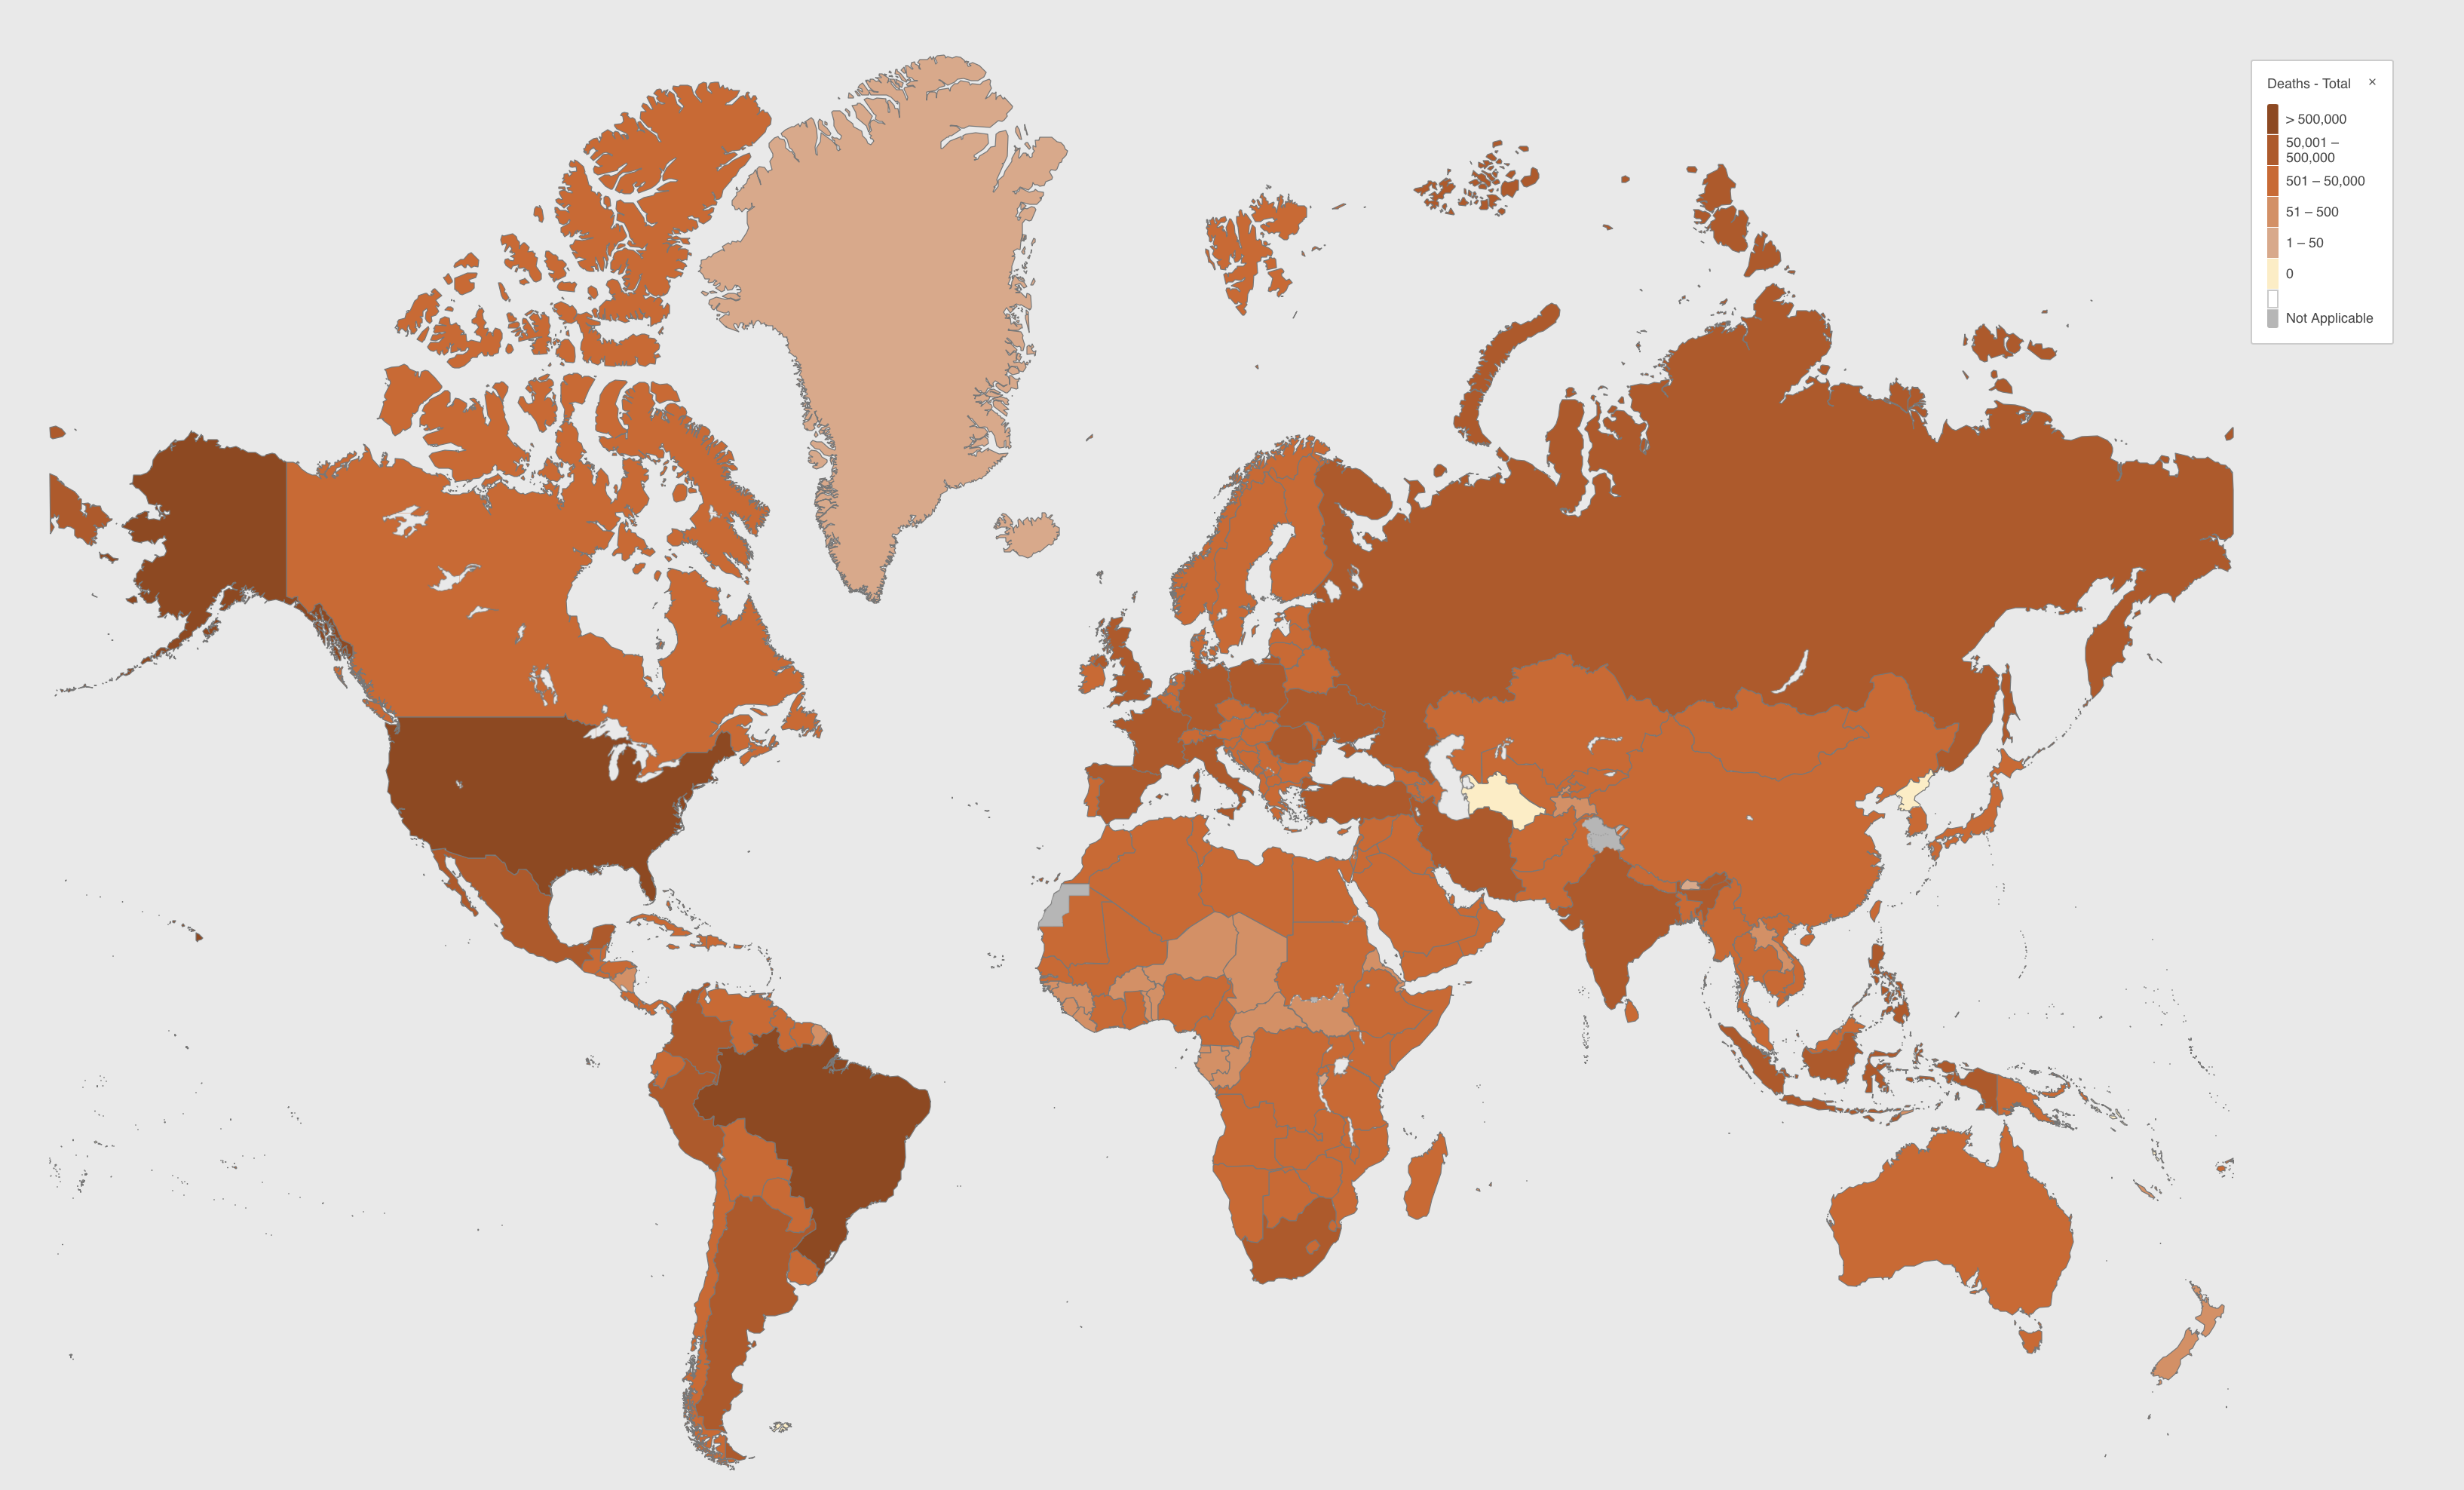
\includegraphics[width = 0.98\textwidth]{Figures_Web/who_totalcases_choro.png}
	\caption{Choropleth map of the COVID-19 cases world-wide by country \citep{WHOCoronavirusCOVID19}.}
	\label{fig:choro1}
\end{figure*}

The issues with choropleth maps were highlighted in trade publications during the initial stages of the pandemic \citep{fieldMappingCoronavirusResponsibly}, but these publications did not penetrate the bureaucracy of public health officials suddenly tasked with data visualisation in real time at scale. 

Proportional symbol maps, see \Cref{fig:propsymb} or graduated symbol maps place scaled symbols or diagrams directly on the input map, often on the centroid of the regions. 
The symbol, most commonly a disk or a square, is scaled such that its area corresponds to the data value of the region. 
Proportional symbol maps sacrifice familiar shapes and topological connectedness for equal visual weight\citep{gaoUsabilityValuebyalphaMaps2019}; while this representation avoids the area bias, proportional symbol maps are subject to under-estimation biases \citep{shimAnalysisMiddleSchool2008} that may be of particular concern when visualizing epidemic disease spread.
In addition, the visual impression of any map based illustration depends on the projection chosen for the underlying map; the examples in \Cref{fig:choro1} and \Cref{fig:propsymb} have a western-centric bias.


\begin{figure*}
	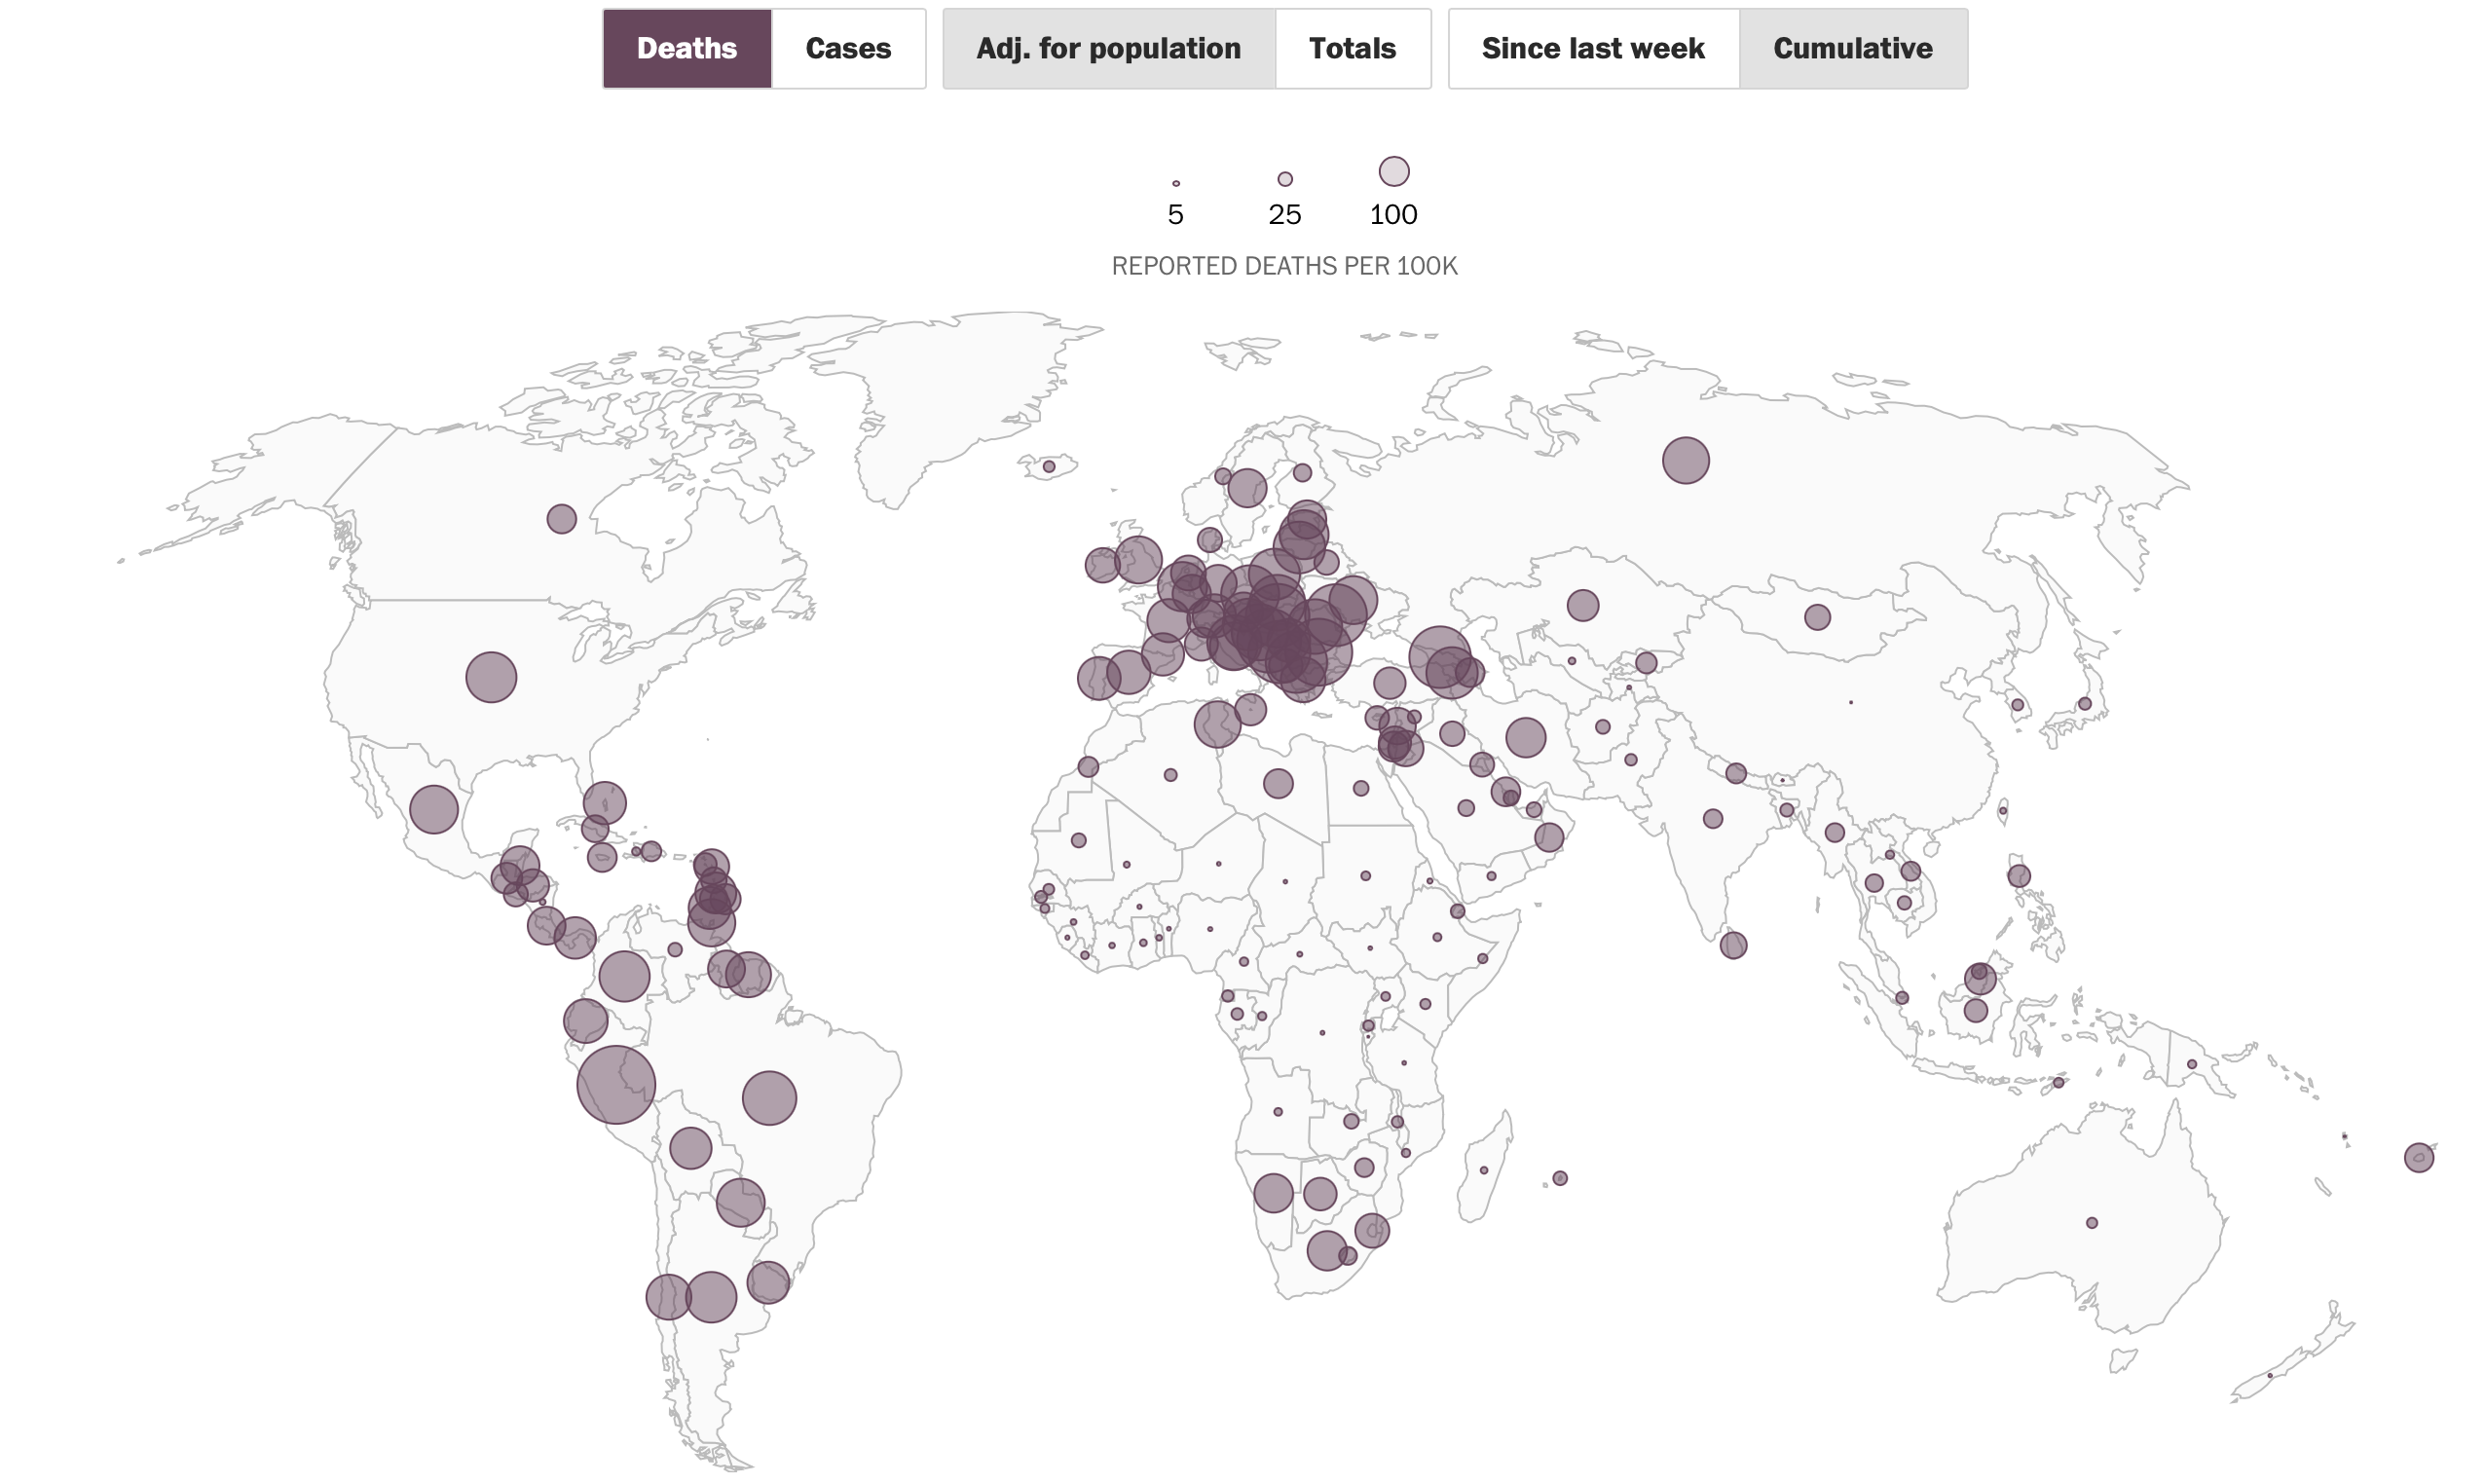
\includegraphics[width = 0.98\textwidth]{Figures_Web/wp_totaldeaths_propsymb.png}
	\caption{Proportional symbol map showing the cumulated reported COVID-19 related deaths adjusted for population world-wide by country \citep{alcantaraMappingWorldwideSpread}.}
	\label{fig:propsymb}
\end{figure*}

Another modification of the standard choropleth to address the area-bias problem is to relax the spatial borders of a region in order to show magnitude using area (as well as colour). Various algorithms can be used to modify geographic boundaries to maintain spatial continuity, or shapes such as hexagons or squares can be used to represent geographic entities (as in \Cref{fig:hex-cartogram}); with either choice, geometry, topology, or both must be sacrificed.  While these methods are more popular in the academic visualisation literature, including analysis of the spread of COVID-19\citep{yalcinMappingGlobalSpatiotemporal2022}, they were not overly common in the media for global representations of COVID information. This may be because cartograms require more visual effort on the part of the viewer; in addition, news organizations may be reluctant to assume their readers have the geographic sophistication necessary to translate between the distorted map of the globe as drawn on the cartogram and the undistorted mental map of the globe used for mental comparison purposes. 
A spatial dot density map might have allowed for analysis of data across geographic boundaries, but this approach was not commonly used to show global case counts, though it was highlighted as a useful option at the national level \citep{fieldMappingCoronavirusResponsibly}, as shown in \Cref{fig:china-dot-map}.

The narrative of the global perspective seems to be highly limited to the aspect of a pandemic affecting the entire globe: none of the above viusalisations intends to provide a deeper insight into the spatial distribution of the phenomenon, neither within the administratively motivated spatial borders nor across them. 
The use of maps to assess the global pandemic more often focuses on the comparative aspects: how are we doing as opposed to our neighbors? Which strategy to fight COVID-19 is better? 
We will examine these topics more closely in \Cref{sec:rankings}.


\begin{figure}
\centering
\begin{subfigure}[c]{\textwidth}
\centering
\includegraphics[width=.65\textwidth]{COVID-tracking-hex-cartogram}
\caption{Hexagonal Cartogram of COVID-19 cases in the United States by state \citep{StateCases1M2021}.}\label{fig:hex-cartogram}
\end{subfigure}

\begin{subfigure}[c]{\textwidth}
\centering
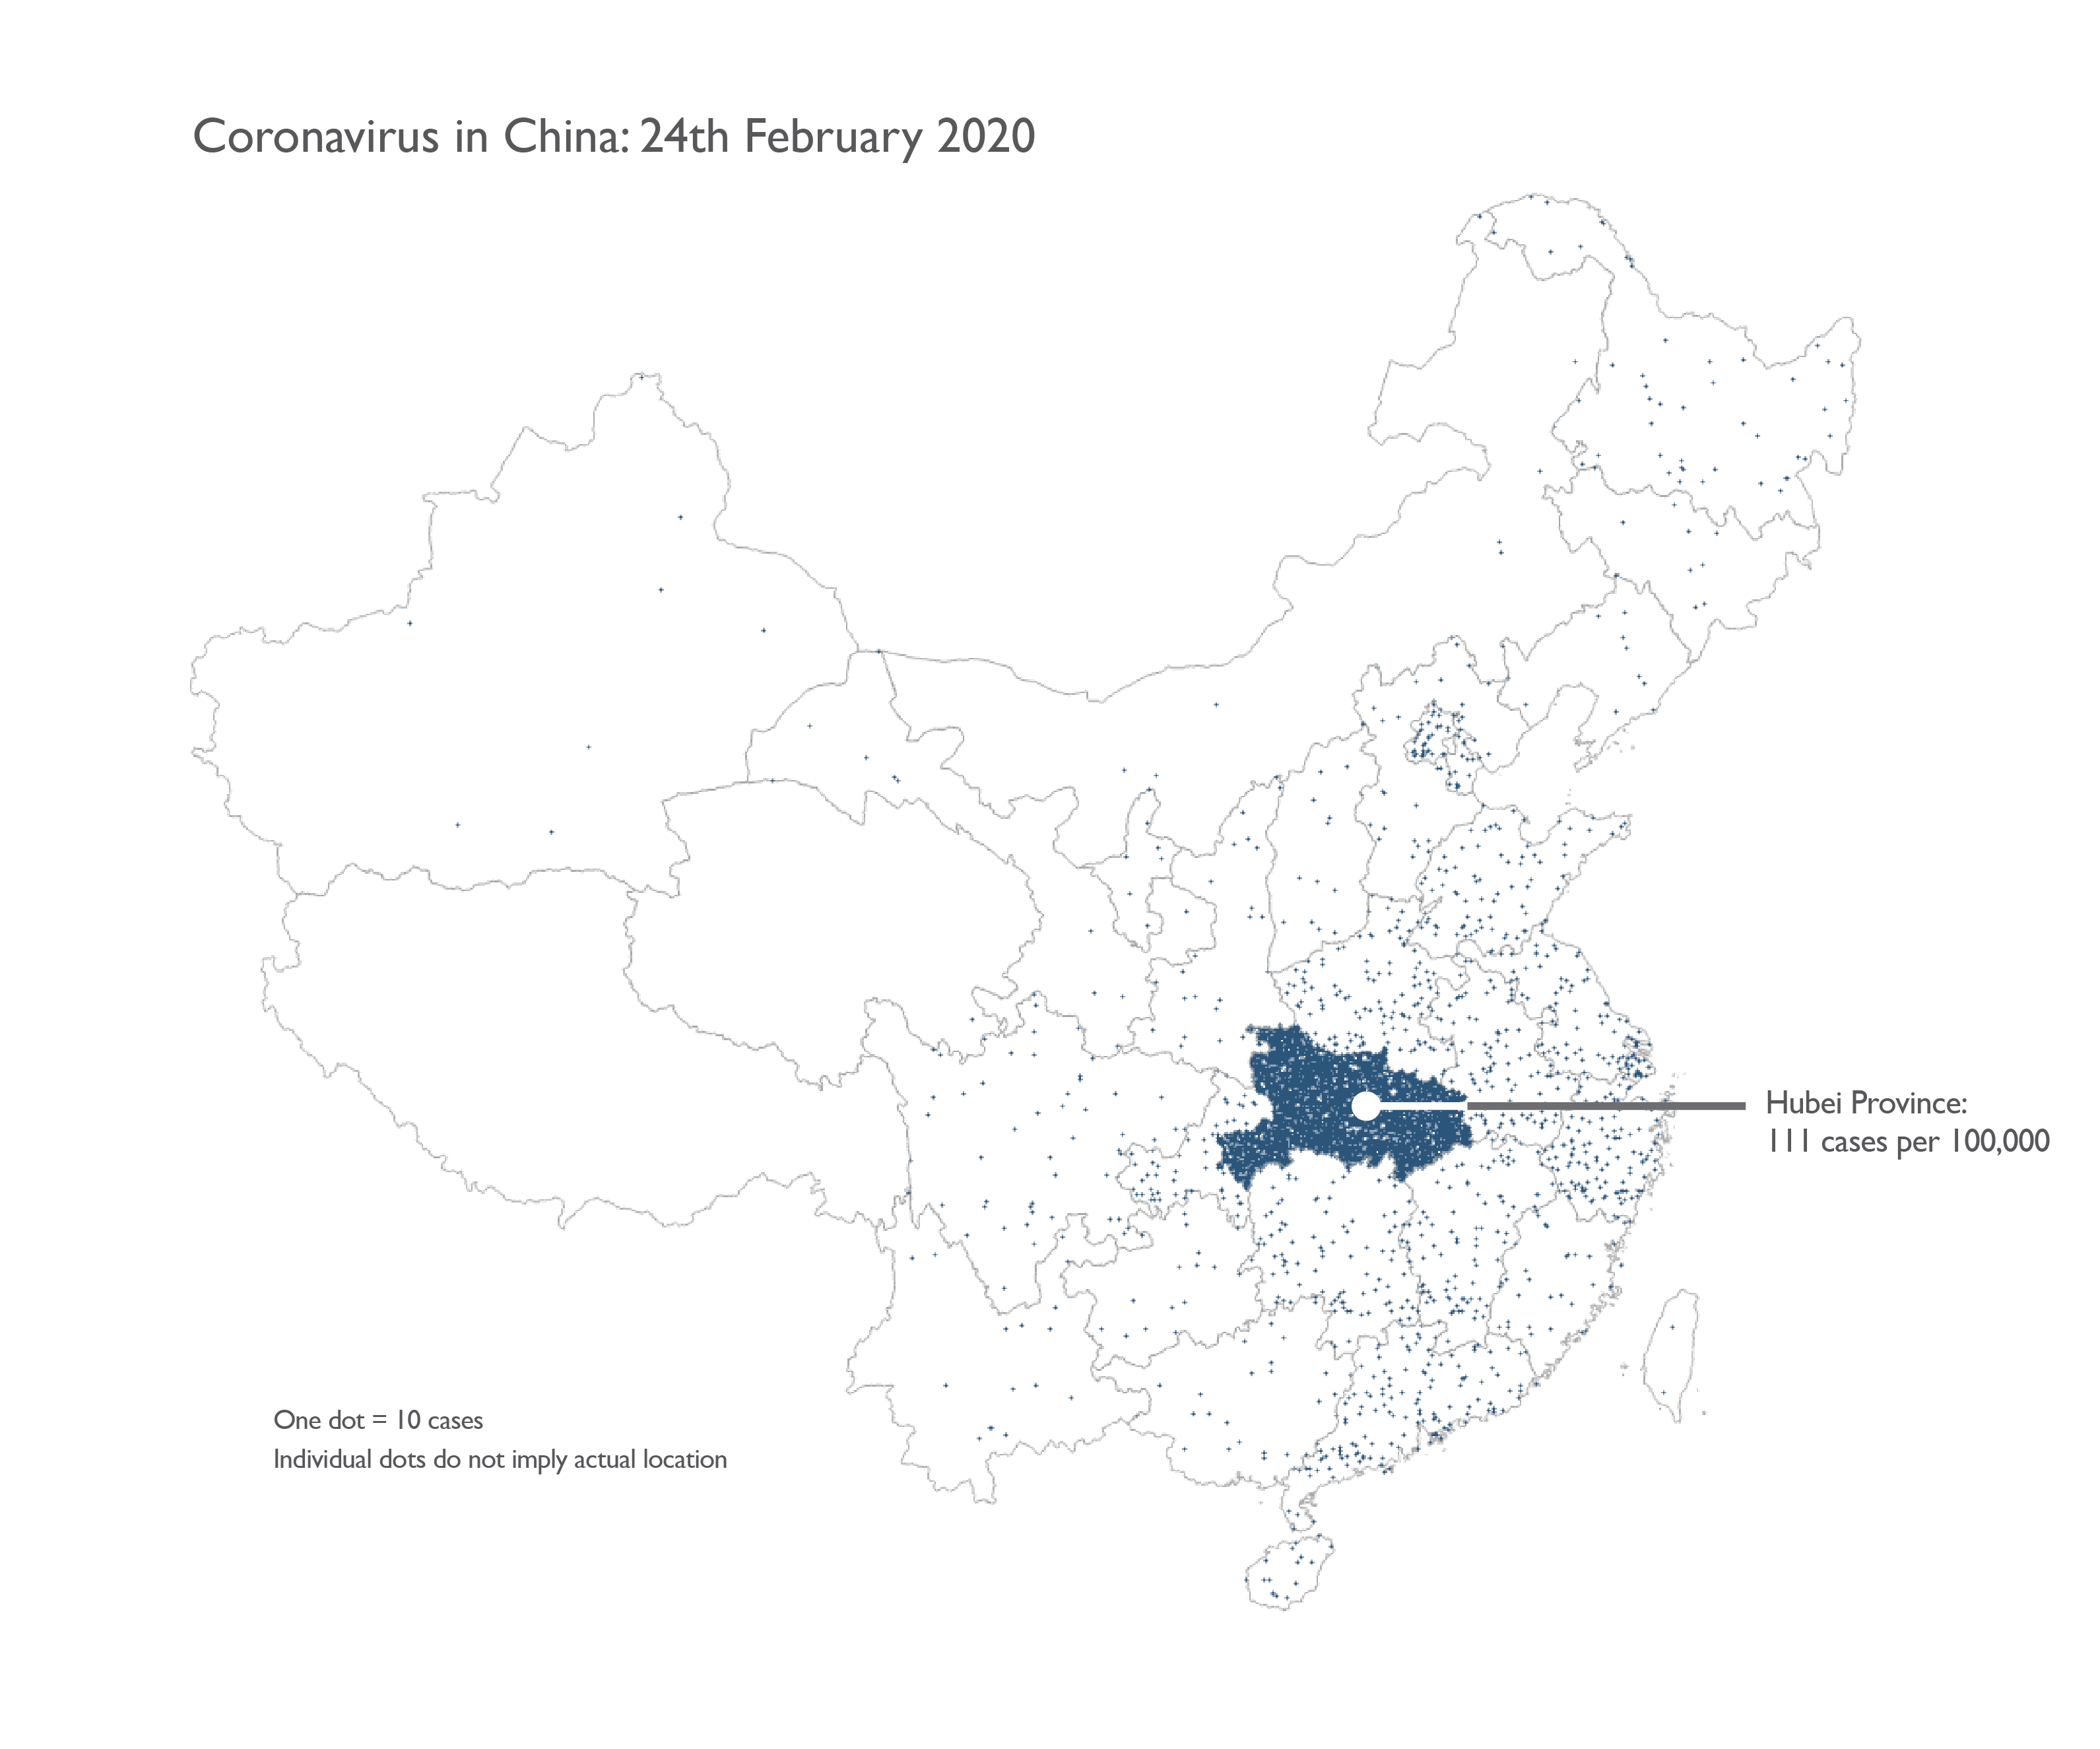
\includegraphics[width=\textwidth]{china-dotmap}
\caption{A dot-density map of COVID cases in China \citep{fieldMappingCoronavirusResponsibly}.}\label{fig:china-dot-map}
\end{subfigure}
% \begin{subfigure}[t]{.45\textwidth}
% \includegraphics[width=\textwidth]{nyt-COVID-scaled-choro}
% \caption{Choropleth Map of COVID cases per country, scaled by population. Source: New York Times \url{https://www.nytimes.com/interactive/2021/world/COVID-cases.html}.}\label{fig:scaled-choro}
% \end{subfigure}
\caption{Modifications of choropleth maps which attempt to address the area bias of choropleths in different ways. Both methods are applied at the national scale rather than at global scale because of limitations with the visual form or data quality.}
\end{figure}
% 
% \begin{minipage}{\linewidth}
% \begin{minipage}{.7\linewidth}
% \includegraphics[width=\textwidth]{COVID-tracking-hex-cartogram}
% \end{minipage}
% \begin{minipage}{.29\linewidth}
% \captionof{figure}{Hexagonal Cartogram of COVID-19 cases in the United States by state. The COVID Tracking Project \url{https://COVIDtracking.com/data/charts/us-daily-positive-cases}.}\label{fig:hex-cartogram}
% \end{minipage}
% \end{minipage}
% 
% \begin{minipage}{\linewidth}
% \begin{minipage}{.7\linewidth}
% 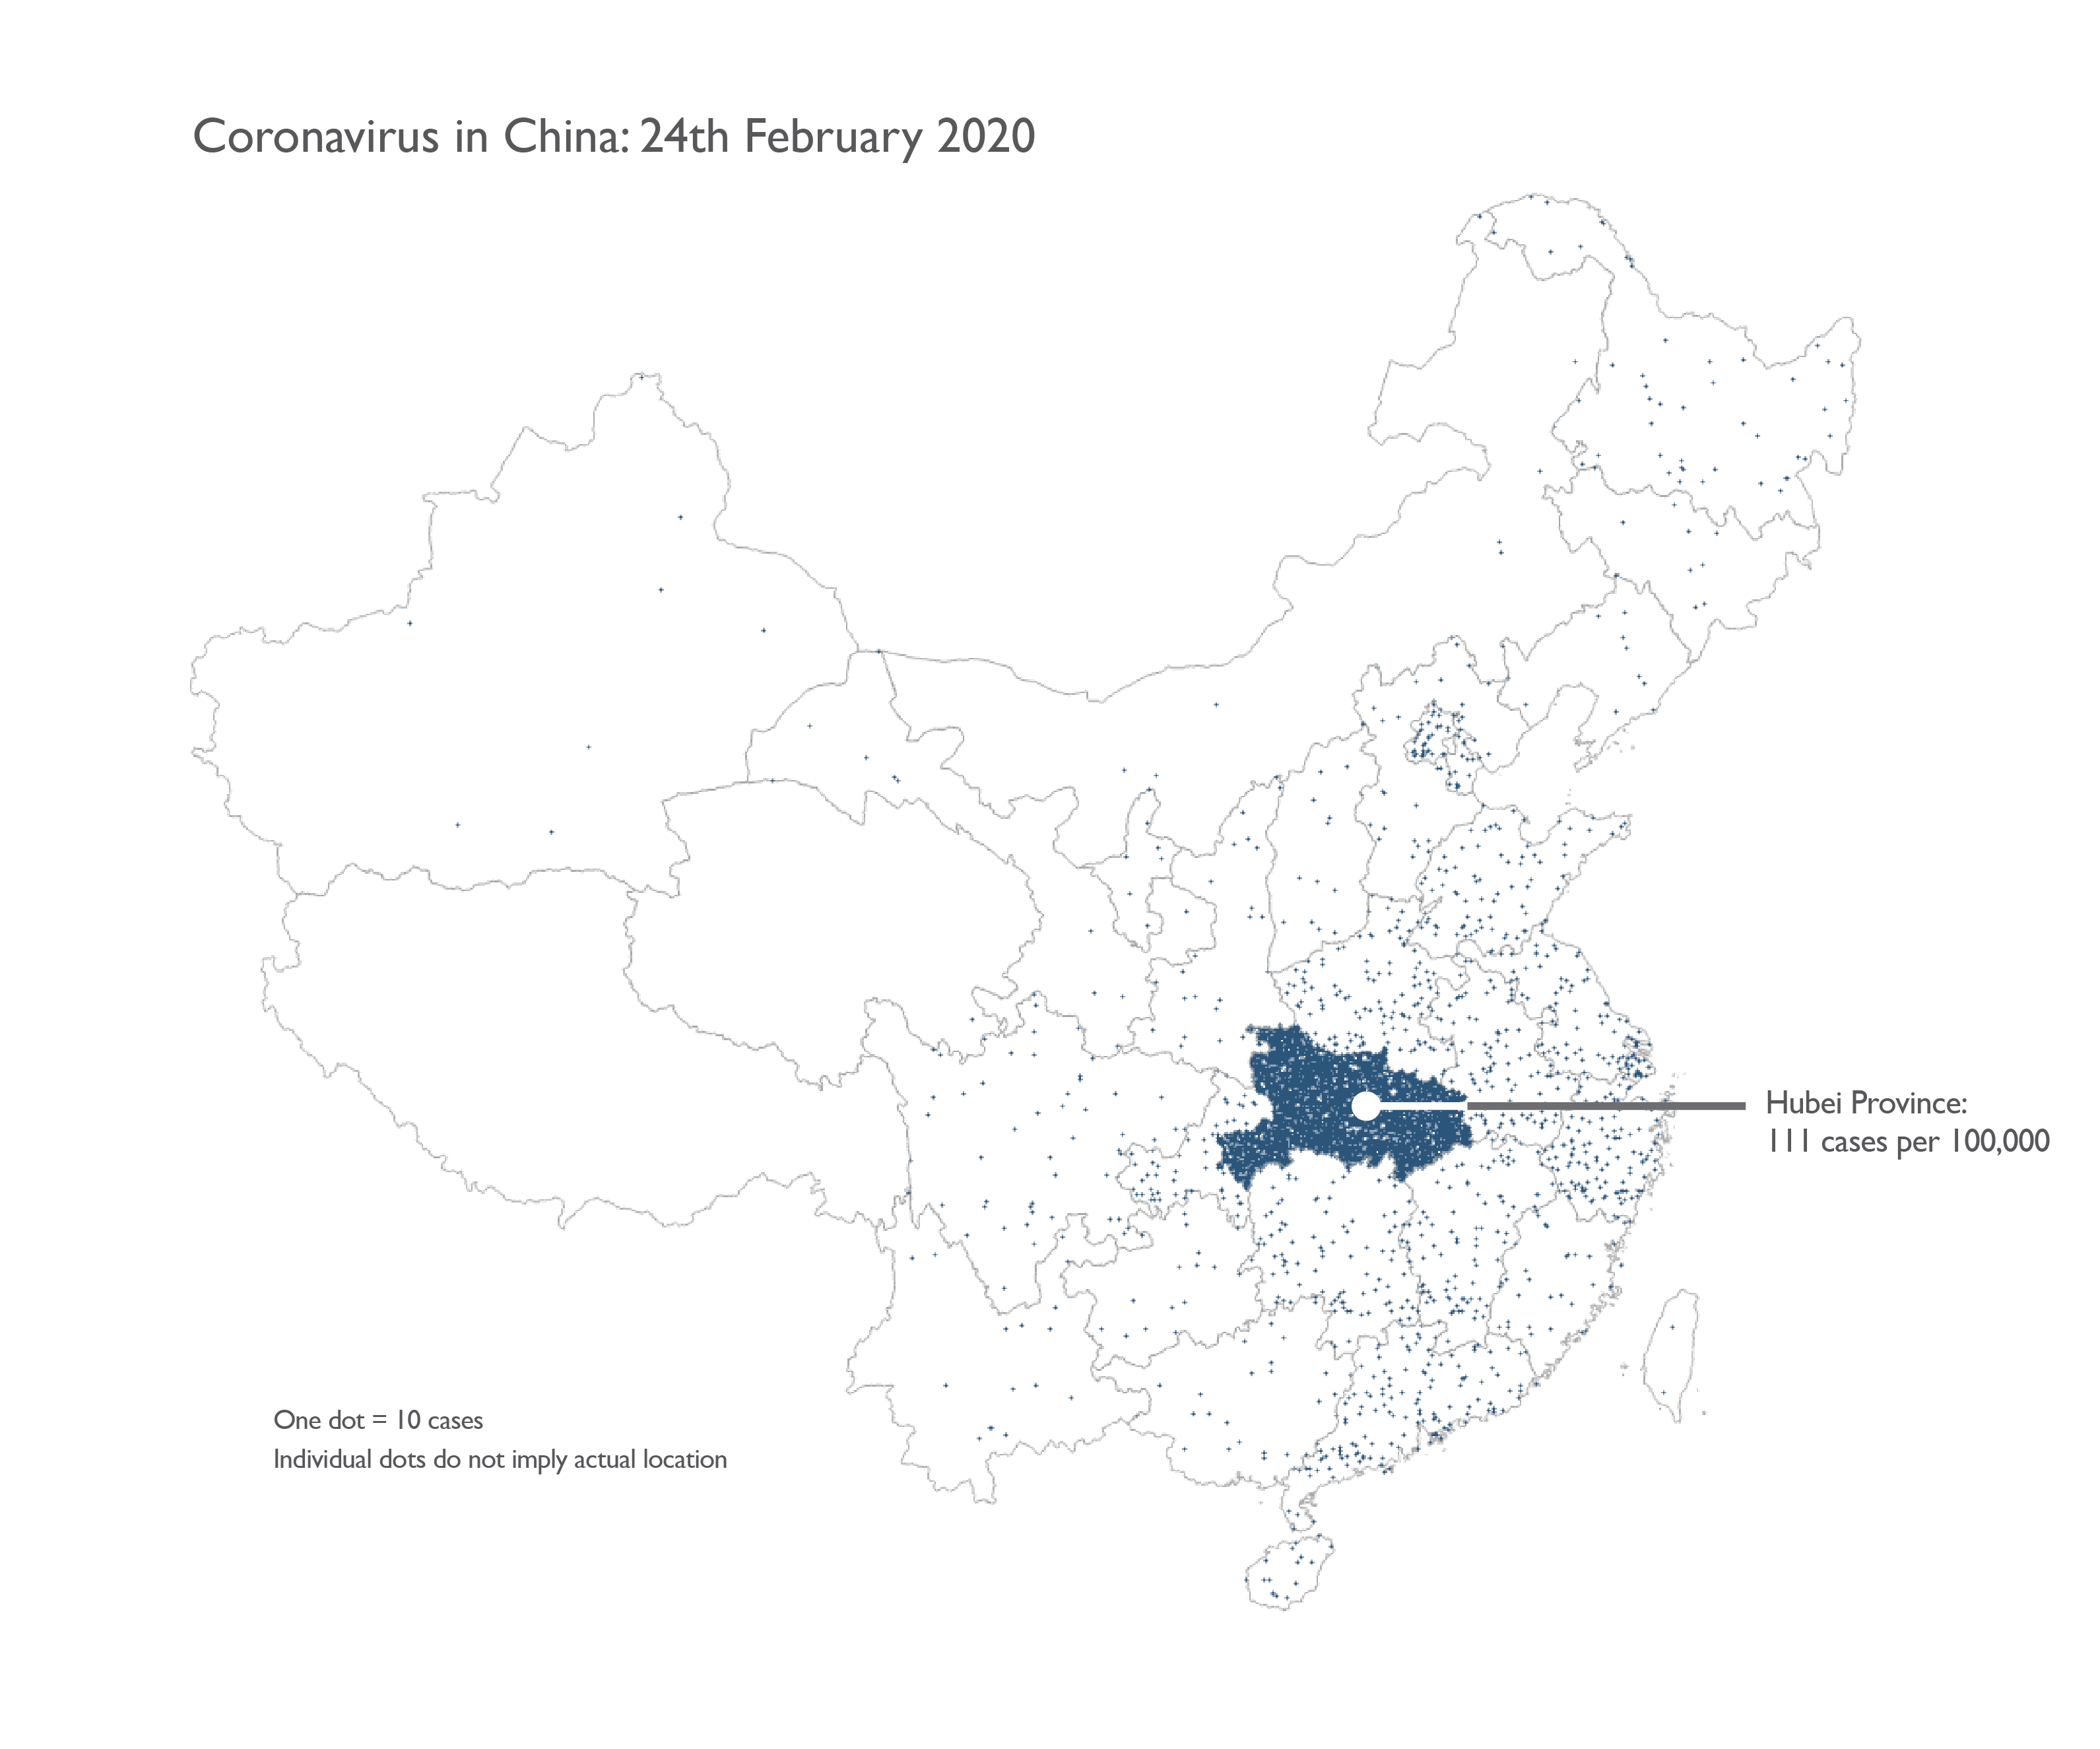
\includegraphics[width=\textwidth]{china-dotmap}
% \end{minipage}
% \begin{minipage}{.29\linewidth}
% \captionof{figure}{A dot-density map of COVID cases in China \citep{fieldMappingCoronavirusResponsibly}.}\label{fig:china-dot-map}
% \end{minipage}
% \end{minipage}




% \begin{figure}
% \centering
% \begin{subfigure}[t]{.45\textwidth}
% \includegraphics[width=\textwidth]{COVID-tracking-hex-cartogram}
% \caption{Hexagonal Cartogram of COVID-19 cases in the United States by state, per million people. This somewhat mitigates the area bias issue, but is still subject to other perceptual biases. Source: The COVID Tracking Project at The Atlantic \url{https://COVIDtracking.com/data/charts/us-daily-positive-cases}.}\label{fig:hex-cartogram}
% \end{subfigure}\hfill
% \begin{subfigure}[t]{.45\textwidth}
% \includegraphics[width=\textwidth]{nyt-COVID-scaled-choro}
% \caption{Choropleth Map of COVID cases per country, scaled by population. Source: New York Times \url{https://www.nytimes.com/interactive/2021/world/COVID-cases.html}.}\label{fig:scaled-choro}
% \end{subfigure}
% \caption{Modifications of choropleth maps which attempt to address the area bias of choropleths in different ways.}
% \end{figure}


Throughout the pandemic, both in choropleth maps and time series graphs, creators have had to grapple with scale. When scales automatically adjust, mental comparisons across time can become misleading, because the colour scale from yesterday does not mean the same thing as it did today, as the range has expanded and the colours have stayed the same. 
It is not that often that day-to-day design changes (or lack thereof) cause fundamental problems with the interpretation of data visualisation, but during the COVID 19 pandemic this situation was both extremely common and had real consequences: people would glance at the current COVID risk map and assume that "red" meant the same thing that it did yesterday, despite the fact that the underlying values had changed\citep{abiadColorDiagramWHOLebanon2020,rubelHeyUpshotNYTCurious2020,matthewsLessonFutzingData2020}. 
One example of this issue over two months of NY Times graphics is shown in \Cref{fig:sparklines-heatmap-nyt}; the overall colour scheme used changes once, but the variable displayed changes (at least) 4 times over the course of a two month period. 


This problem is more noticeable in choropleths and other charts which show case counts based on colour scale alone than in time series charts, where we are more likely to expect and notice a scale change, but it is still a fundamental issue across chart types and of particular concern when there is no natural upper bound on the variable displayed. 
Some designers leaned into this by arranging their graphics to highlight the fact that cases were ``off the charts", as in \Cref{fig:jbm-tweet}, implicitly cuing readers that the situation was exceptional and worthy of their attention.

\begin{figure}
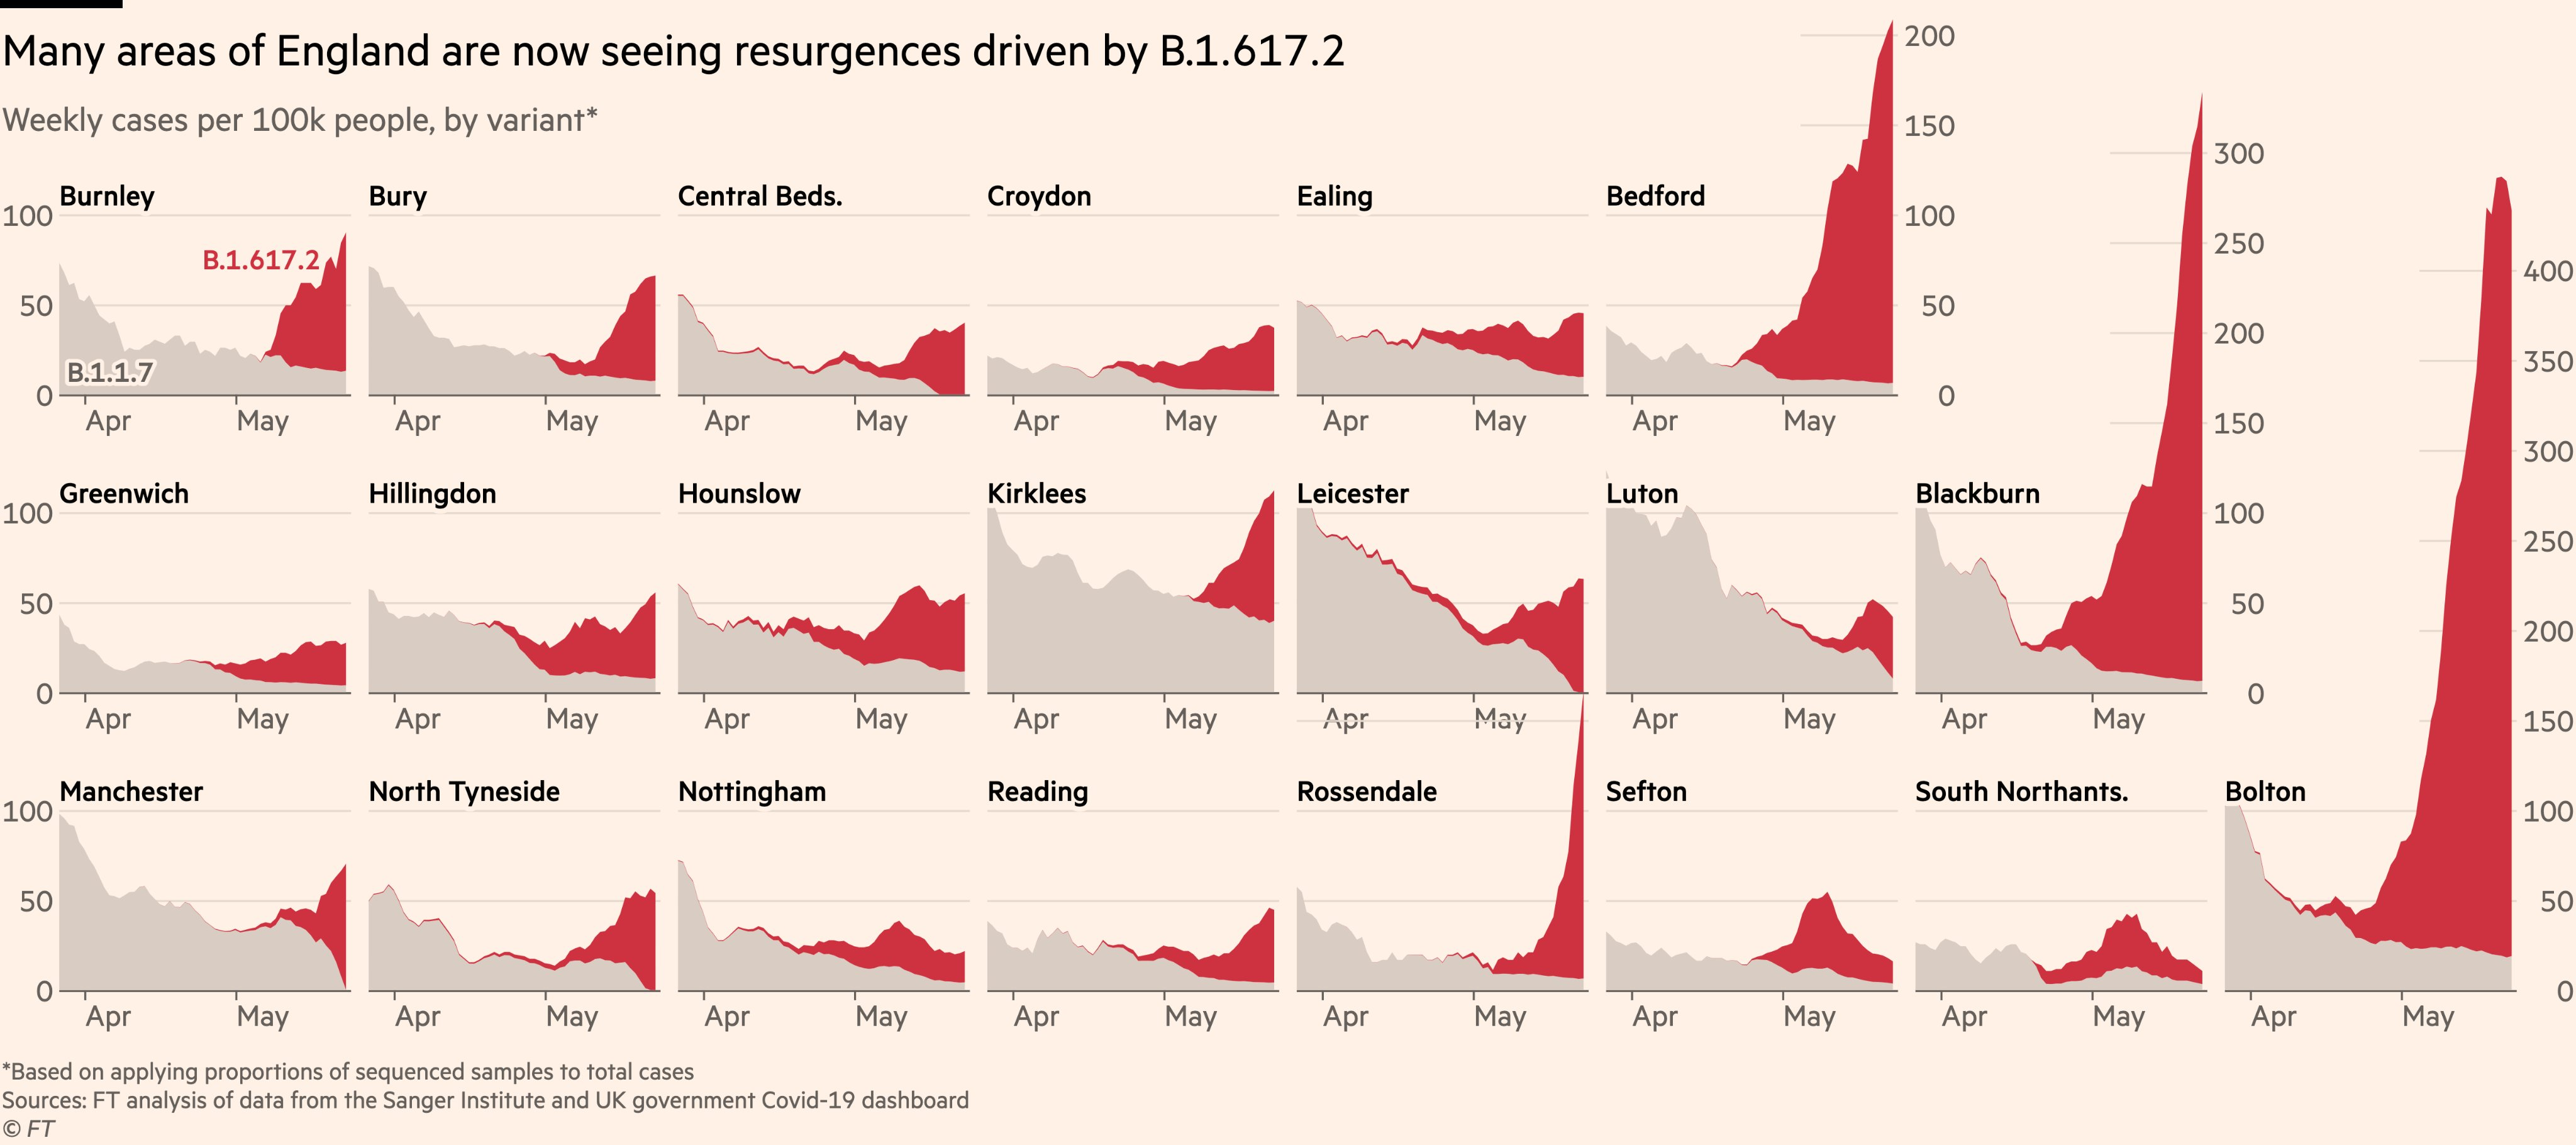
\includegraphics[width=.99\linewidth]{ft-off-charts}
\caption{Chart showing the increase in cases as a result of the B.1.617.2 variant in regions of the UK, May 27, 2021. Notably, this chart arranges areas to accommodate certain regions whose cases are ``off the chart" in order to emphasize the exceptional situation. \citep{burn-murdochNEW1617Fuelling2021}}
\label{fig:jbm-tweet}
\end{figure}

Early in the pandemic, as case numbers grew exponentially without appropriate public health measures to restrain them, the scale problem for choropleth maps was particularly complex: over time either the colour mapping changes or the map becomes useless due to compression against the upper limits of the scale, as in \citet{panchadsaramIfWeAre2020}. 
The magnitude of the problem also depends on whether the scale uses a set of bins (a discrete mapping to a continuous variable) or uses a continuous colour mapping; in some cases, outlets switched between the two options over time or changed the underlying unit entirely. 
Interestingly, media outlets and municipal dashboards were subject to criticism when the colour scales changed in response to increasing case counts\citep{boeckDataVizDecisionmakingAction2020} as well as when the colour scale did not change\citep{sandalowChiTribGraphicsPleaseUpdate2020}, illustrating the difficulty of designing visualisations amid competing constraints and a constantly evolving pandemic.


% Is it worth discussing e.g. https://www.nytimes.com/interactive/2021/us/COVID-risk-map.html that does not make this distinction and runs into the "boy who cried wolf" problem? When everything is always extremely high risk we just tend to tune things out. I don't want to distract from the overview, though... https://twitter.com/rypan/status/1282020934044401664 is a good example




\section{The temporal narrative}
% Line plots, frequency domain, NY times tile plots w/ cases represented in colour intensity

Visualisations are typically created for a specific purpose, and during a pandemic it is particularly critical to show the evolution of the situation over time, as there are new developments on a daily basis. 
Typically, this means that cases, hospitalizations, and/or deaths are plotted on the y-axis, with date shown on the x-axis, as in \Cref{fig:jbm-tweet} and \Cref{fig:wapo-COVID-time-series}. 
This not only allows individuals to compare the present to past case counts, but also allows for forecasting and prediction of the future based on the current state. 
Time series plots are the most natural choice for these goals, and over the course of the pandemic, many different attempts have been made to show time series information using different graphical forms. 

\begin{figure}
\centering
\includegraphics[width=.99\linewidth]{wapo-COVID-monitoring}
\caption{COVID monitoring summary charts on the Washington Post's Coronavirus page \citep{Coronavirus2022}.}
\label{fig:wapo-COVID-time-series}
\end{figure}

The most obvious time series plot is also the most common: plotting cases against date, often with a 7 or 14-day smooth to handle periodicity in case reporting due to the work week, as shown in \Cref{fig:wapo-COVID-time-series}. This allows for individuals to assess the current situation and easily compare the current number of cases to past times for which the individual has a direct reference for what to expect in impact to daily life. Often, as in \Cref{fig:wapo-COVID-time-series}, these time series show multiple variables: cases, deaths, and hospitalizations (and sometimes vaccinations) to provide a more comprehensive view of the situation; this is particularly useful as there has been some decoupling of case numbers and hospitalizations/deaths with the emergence of effective vaccinations and strains which are more contagious but potentially also less severe. Many outlets also provide additional charts designed to provide some immediate context to readers, as shown in \Cref{fig:wapo-context}. 

\begin{figure}
\centering
\includegraphics[width=.5\linewidth]{wapo-COVID-context}
\caption{Some outlets provide contextual information to assist readers with interpreting time series plots \citep{CoronavirusCasesTracking2022}.}
\label{fig:wapo-context}
\end{figure}

However, there are some limitations with this presentation; if we are interested in showing the change in counts over time, viewers must assess the slope of the line, rather than its position. We know that slope judgments are much less accurate than position \citep{clevelandGraphicalPerceptionVisual1987}, even in relatively simple situations; when we add in our ability to assess exponential growth, our perceptual accuracy is even more suspect. This issue will be discussed further in \Cref{sec:logs} when we discuss log scales, which are one solution to our misperception of exponential growth.

Yet another approach to showing the temporal component of the pandemic was to leverage web graphics to show the temporal component through animation; this freed up the $x$ axis which in the default configuration would have been devoted to time and allowed another variable to be displayed. While this approach was common on social media, it was reserved for specific use-cases and more carefully selected variables by professional media outlets. \Cref{fig:bubble-ft} shows an example from the Financial Times which uses the x-axis to show GDP per capita and the y-axis to show vaccination rate, bubble size indicates a country's population. With so many variables and ratios of variables, these charts are complex to read and use, even though they are visually appealing.

\begin{figure}
\centering
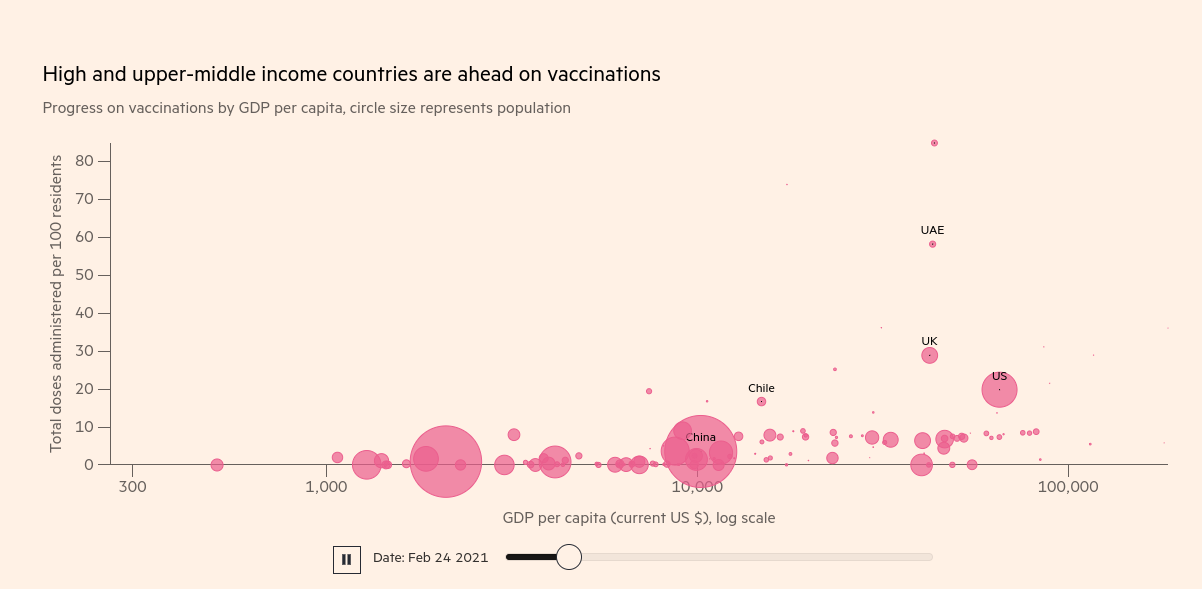
\includegraphics{ft_vaccine_bubble}
\caption{Animated bubble chart showing vaccination rate relative to per capita GDP for each country \citep{visualCovid19VaccineTracker}.}\label{fig:bubble-ft}
\end{figure}

Other time series representations were more abstract, sacrificing exact data representations for a higher-level summary comparing regions and points in time without the burden of numerical calculations. Several versions from the New York Times are shown in \Cref{fig:sparklines-heatmap-nyt}. The advantage of these displays is that they are very simple and allow for viewers to gain an intuitive understanding of the data, however, they do not present precise numerical information and even the colour scale is (perhaps intentionally) opaque -- it would be extremely difficult to translate the visualisation into any sort of accurate numerical estimate. In addition, by hiding these details from the user, it is very difficult to identify when the underlying mathematical representation changes over time, as it did several times during the summer of 2020. The use of a similar colour scheme as well as similar geometric representations made it extremely difficult for users to identify that the value represented had changed. Clearly, the purpose of these charts is not to provide numerical precision, but rather a comparative assessment of the status of one region relative to others as well as relative to previous time points. 

% 
% \begin{figure}
% \centering
% 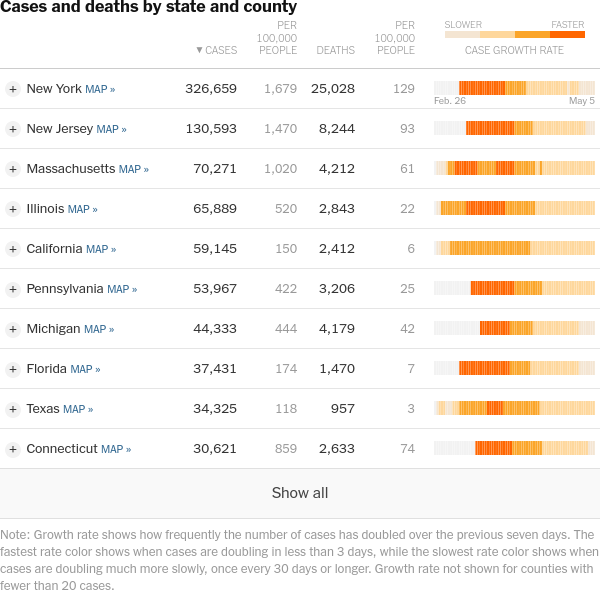
\includegraphics[width=.3\linewidth]{NYT-heatmap-crop}\hfill
% 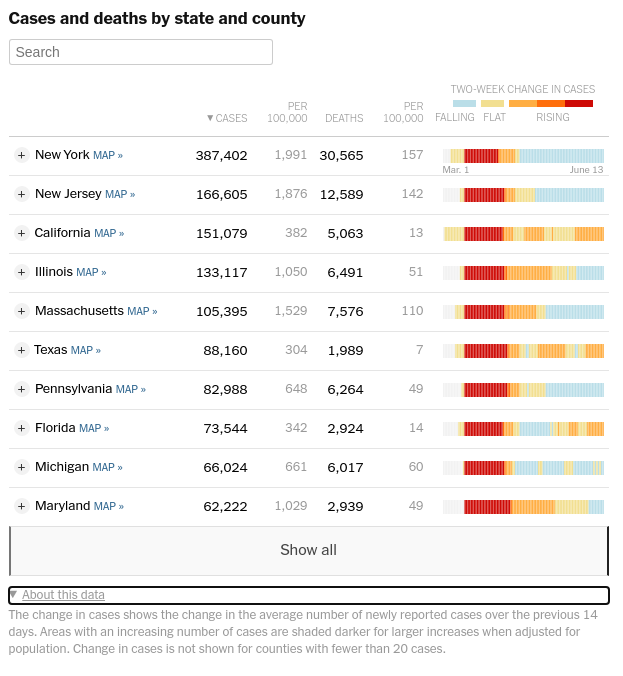
\includegraphics[width=.3\linewidth]{NYT-heatmap-crop3}\hfill
% 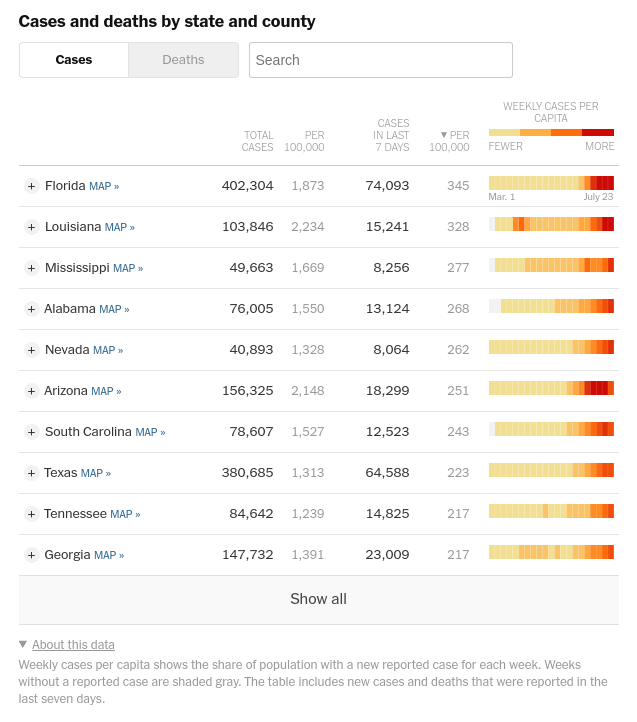
\includegraphics[width=.3\linewidth]{NYT-heatmap-crop2}
% \caption{Sparklines style heatmaps embedded in a table of coronavirus data by state. Over the course of Summer 2020, the specific measures shown changed, even though the form of the data remained highly similar. Source: \url{https://www.nytimes.com/interactive/2020/us/coronavirus-us-cases.html} (May 6, 2020; June 15, 2020; and July 24, 2020, respectively) }
% 
% \label{fig:sparklines-heatmap-nyt}
% \end{figure}

\begin{figure}
\centering
\begin{subfigure}[t]{.25\textwidth}
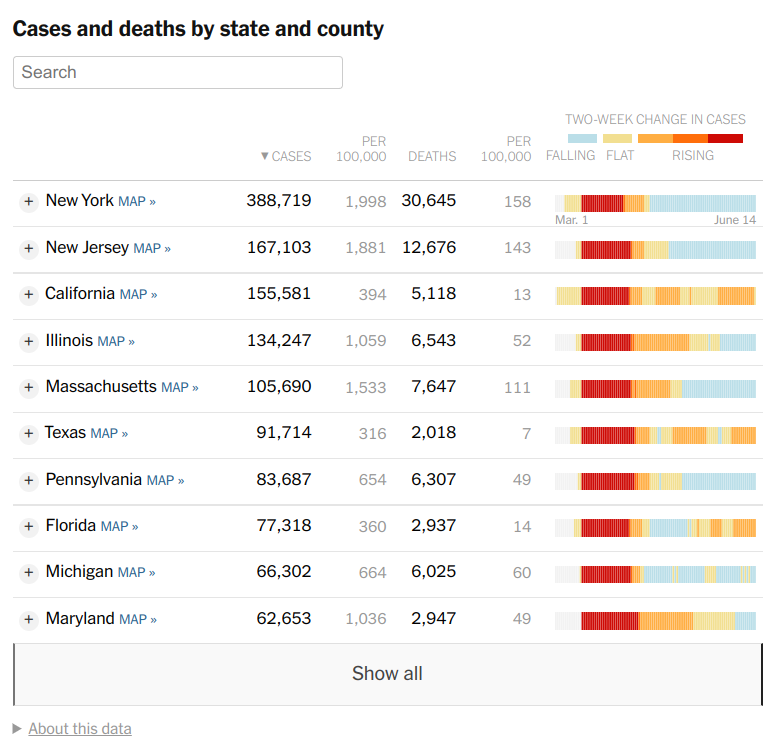
\includegraphics[width=\textwidth]{nyt-wayback-20200616}
\caption{June 16, 2020}\label{fig:nyt-colors1}
\end{subfigure}\hfill
\begin{subfigure}[t]{.25\textwidth}
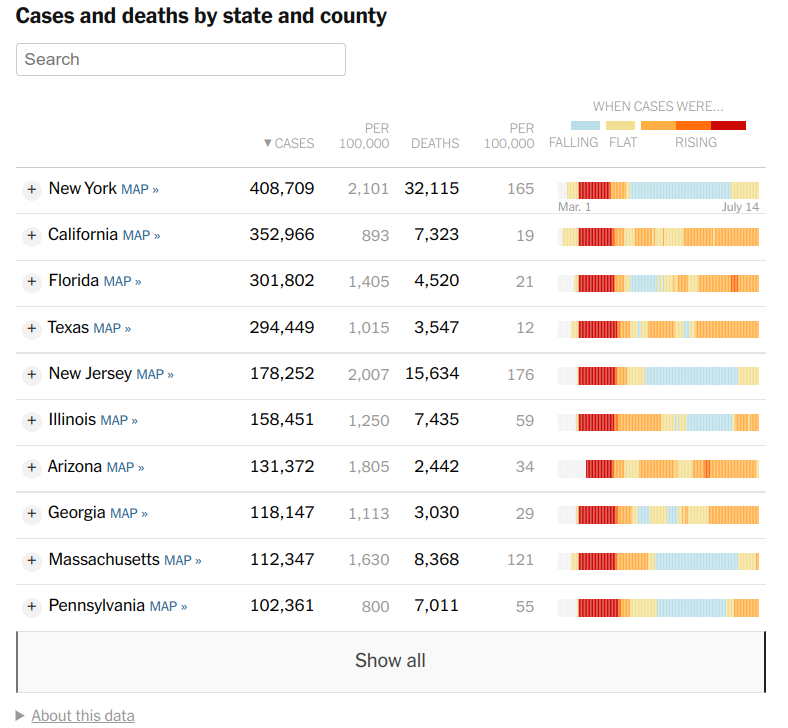
\includegraphics[width=\textwidth]{nyt-wayback-20200716}
\caption{July 16, 2020}\label{fig:nyt-colors2}
\end{subfigure}\hfill
\begin{subfigure}[t]{.25\textwidth}
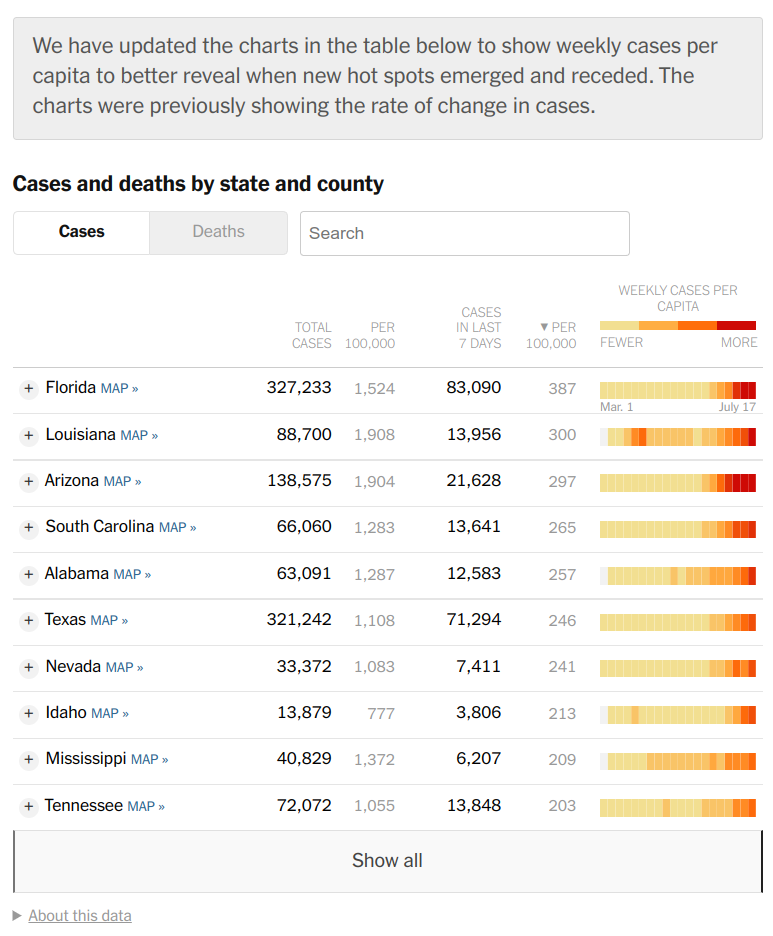
\includegraphics[width=\textwidth]{nyt-wayback-20200718}
\caption{July 18, 2020}\label{fig:nyt-colors3}
\end{subfigure}\hfill
\begin{subfigure}[t]{.25\textwidth}
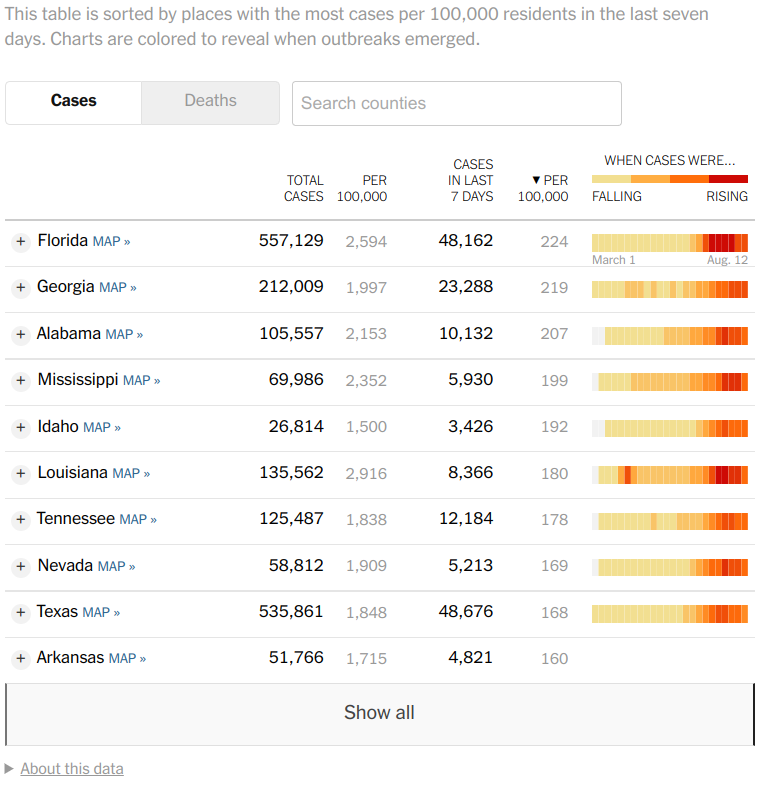
\includegraphics[width=\textwidth]{nyt-wayback-20200814}
\caption{August 1, 2020}\label{fig:nyt-colors4}
\end{subfigure}\hfill
\caption{A series of screenshots of the NY Times state-by-state display showing evolving colour schemes and even metrics; initially, a discrete scale of two-week change in cases is shown; then, a similar colour scheme is used with a different metric. Around July 17, the colour scheme and variable shown changed to weekly cases per capita (from "fewer" to "more"), and by August 14, the variable shown changed back again ("falling" to "rising") while the colour scheme stayed the same.}\label{fig:sparklines-heatmap-nyt}
\end{figure}

One unique time series plot created a representation of the case counts in the frequency domain; instead of plotting cases as they occurred, the chart instead shows line segments from 0 to N in $y$, where $N$ is a predefined number of cases; then the chart resets to show the next angle. This produces a sense of intensity of the waves of the pandemic over time as shown in \Cref{fig:freq-domain}. Interestingly, this frequency representation can also be easily transferred into an audio domain, providing access for visually impaired users as well as a multimodal representation of the data for sighted users. 

\begin{figure}
\centering
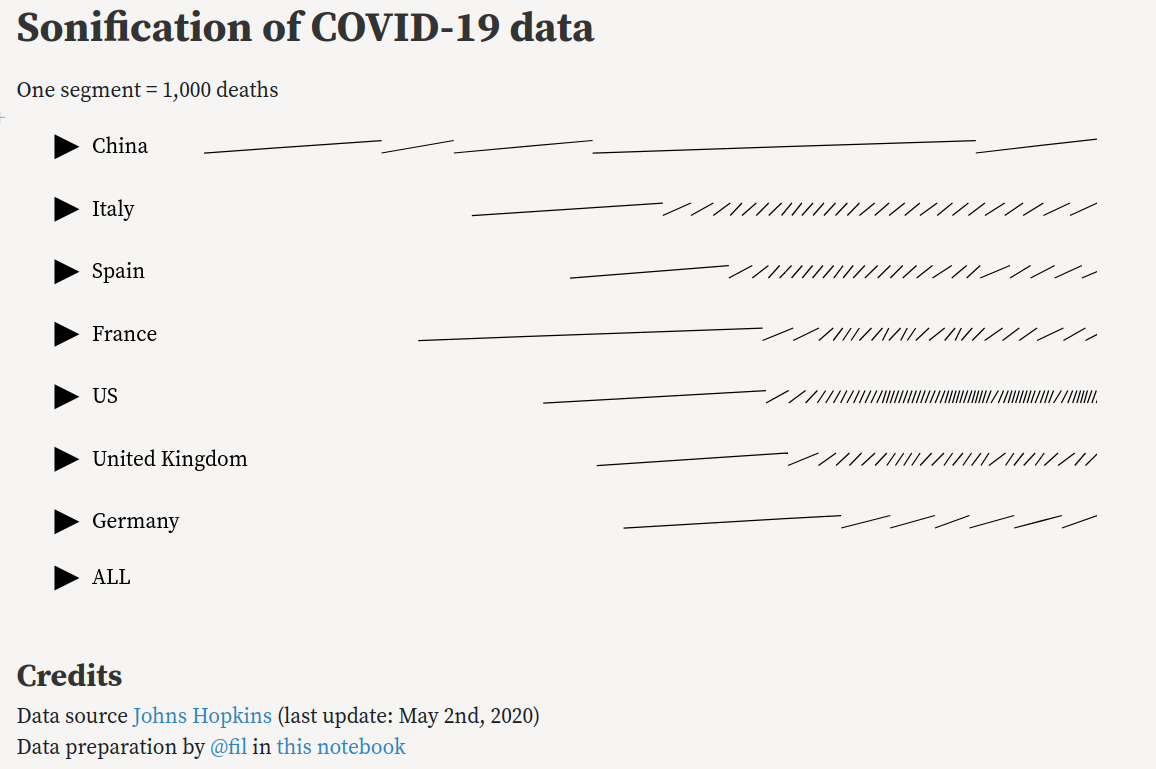
\includegraphics[width=.75\linewidth]{frequency-domain}
\caption{Frequency-domain case count graphics. Here, each 1000 deaths are represented by a single line segment whose slope represents the time taken to reach the next 1000 deaths. This provides viewers with a sense of the pace of the epidemic, rather than the raw case counts in more standard time series representations. This representation can also be shown in the auditory domain, providing access to those who are typically excluded from visualisations due to vision loss \citep{vuillemotSonificationCOVID19Data2020}.}
\label{fig:freq-domain}
\end{figure}

There are many different ways that designers can use time series data to provide additional contextual information and facilitate comparisons. \Cref{fig:ft-waves} shows COVID cases, positivity rate, and hospital admissions from South Africa's Gauteng province, which was one of the first areas to experience a large wave of the Omicron variant. This chart provides context for the Omicron wave, showing that while infections are occurring at a much faster rate than in previous waves, hospital admissions seem to be approximately following previous trends. In addition, it is clear that the chart is highlighting the Omicron variant from the colour selection: the red used to show the Omicron numbers is a sharp contrast from the green and blue shades used to show the first three waves of the pandemic. Notably, even though red and green in combination are usually to be avoided for the sake of colourblind viewers, the shades of blue/green variants which are chosen are light enough that the red stands out even to someone with colour vision deficiency.

\begin{figure}\centering
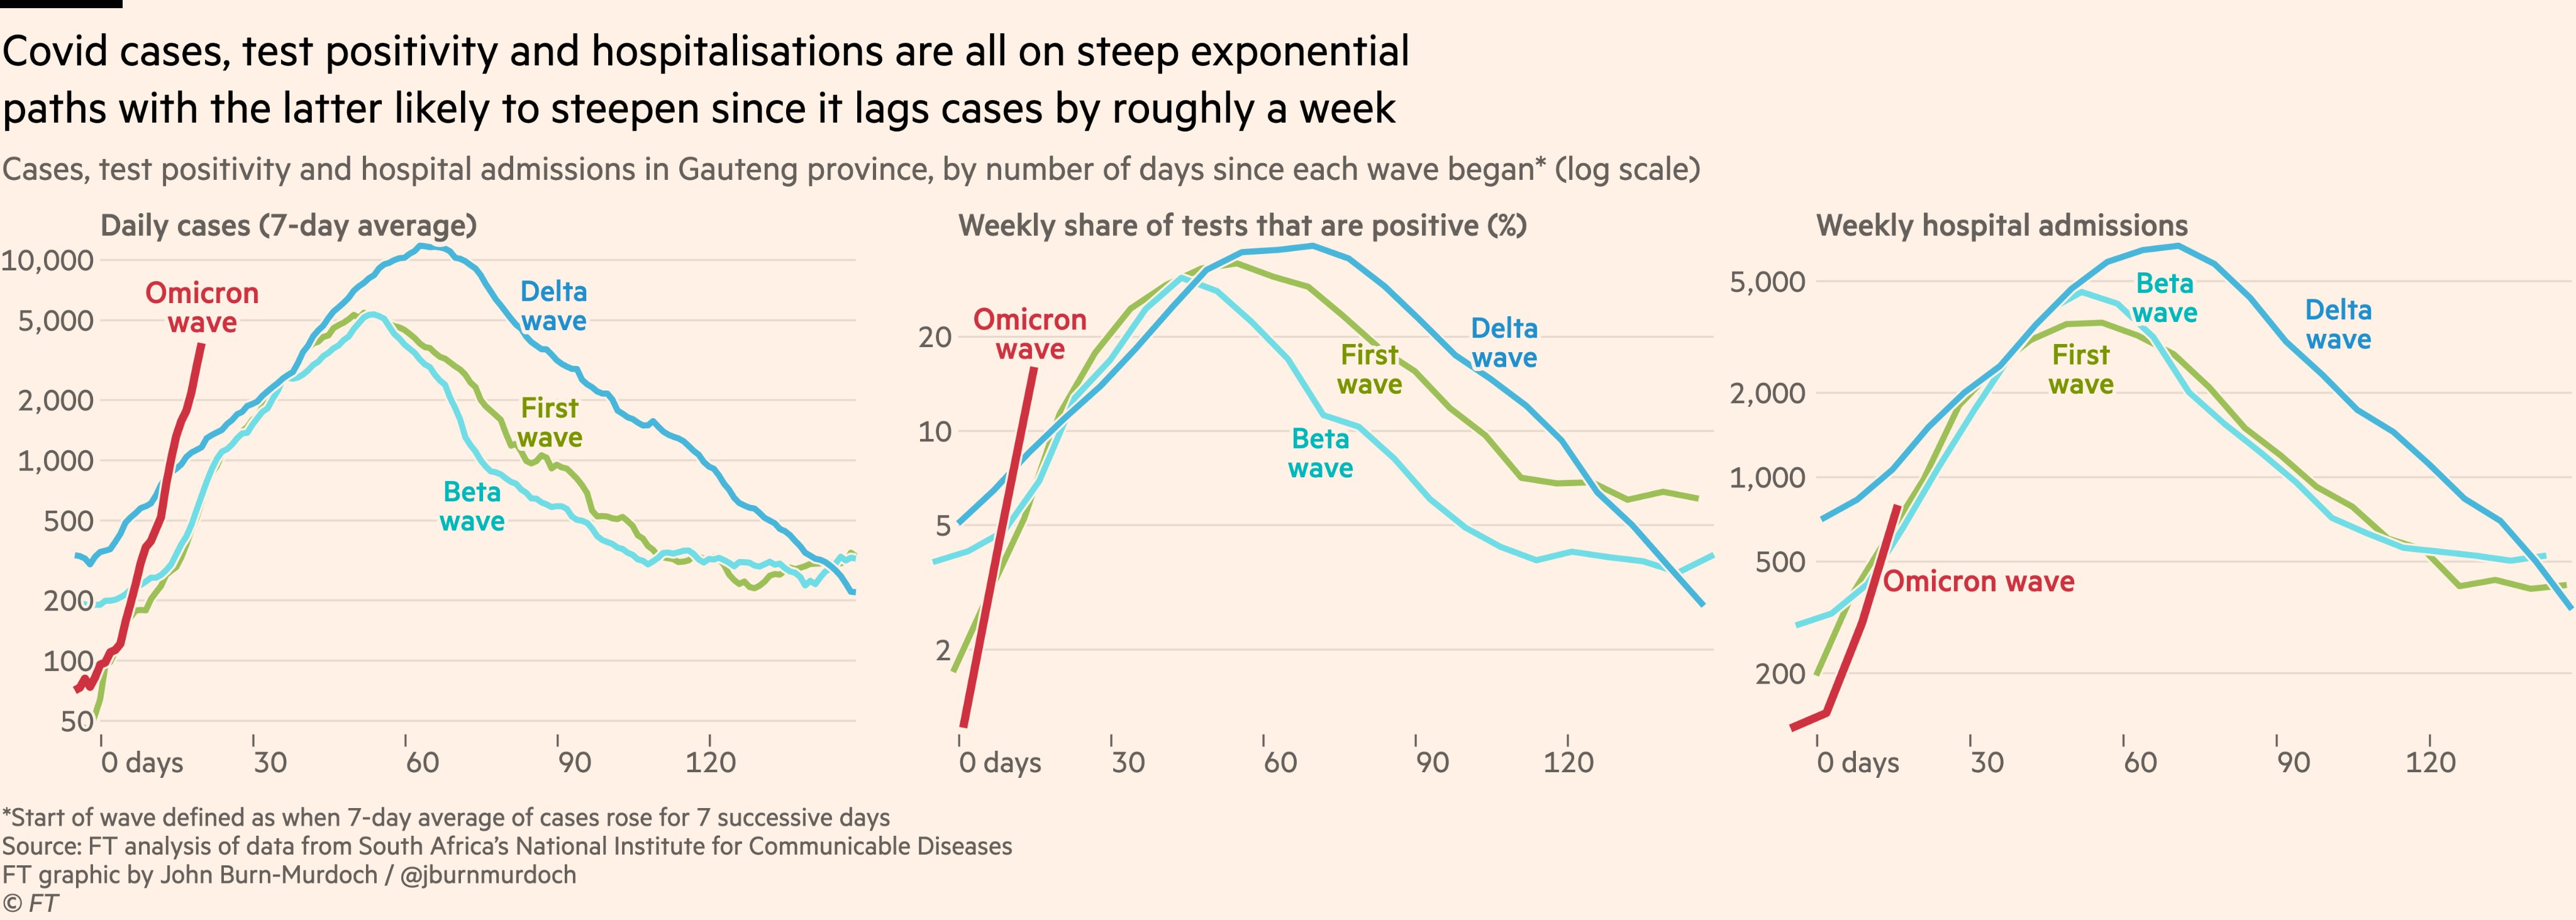
\includegraphics[width=\linewidth]{ft-waves}\\
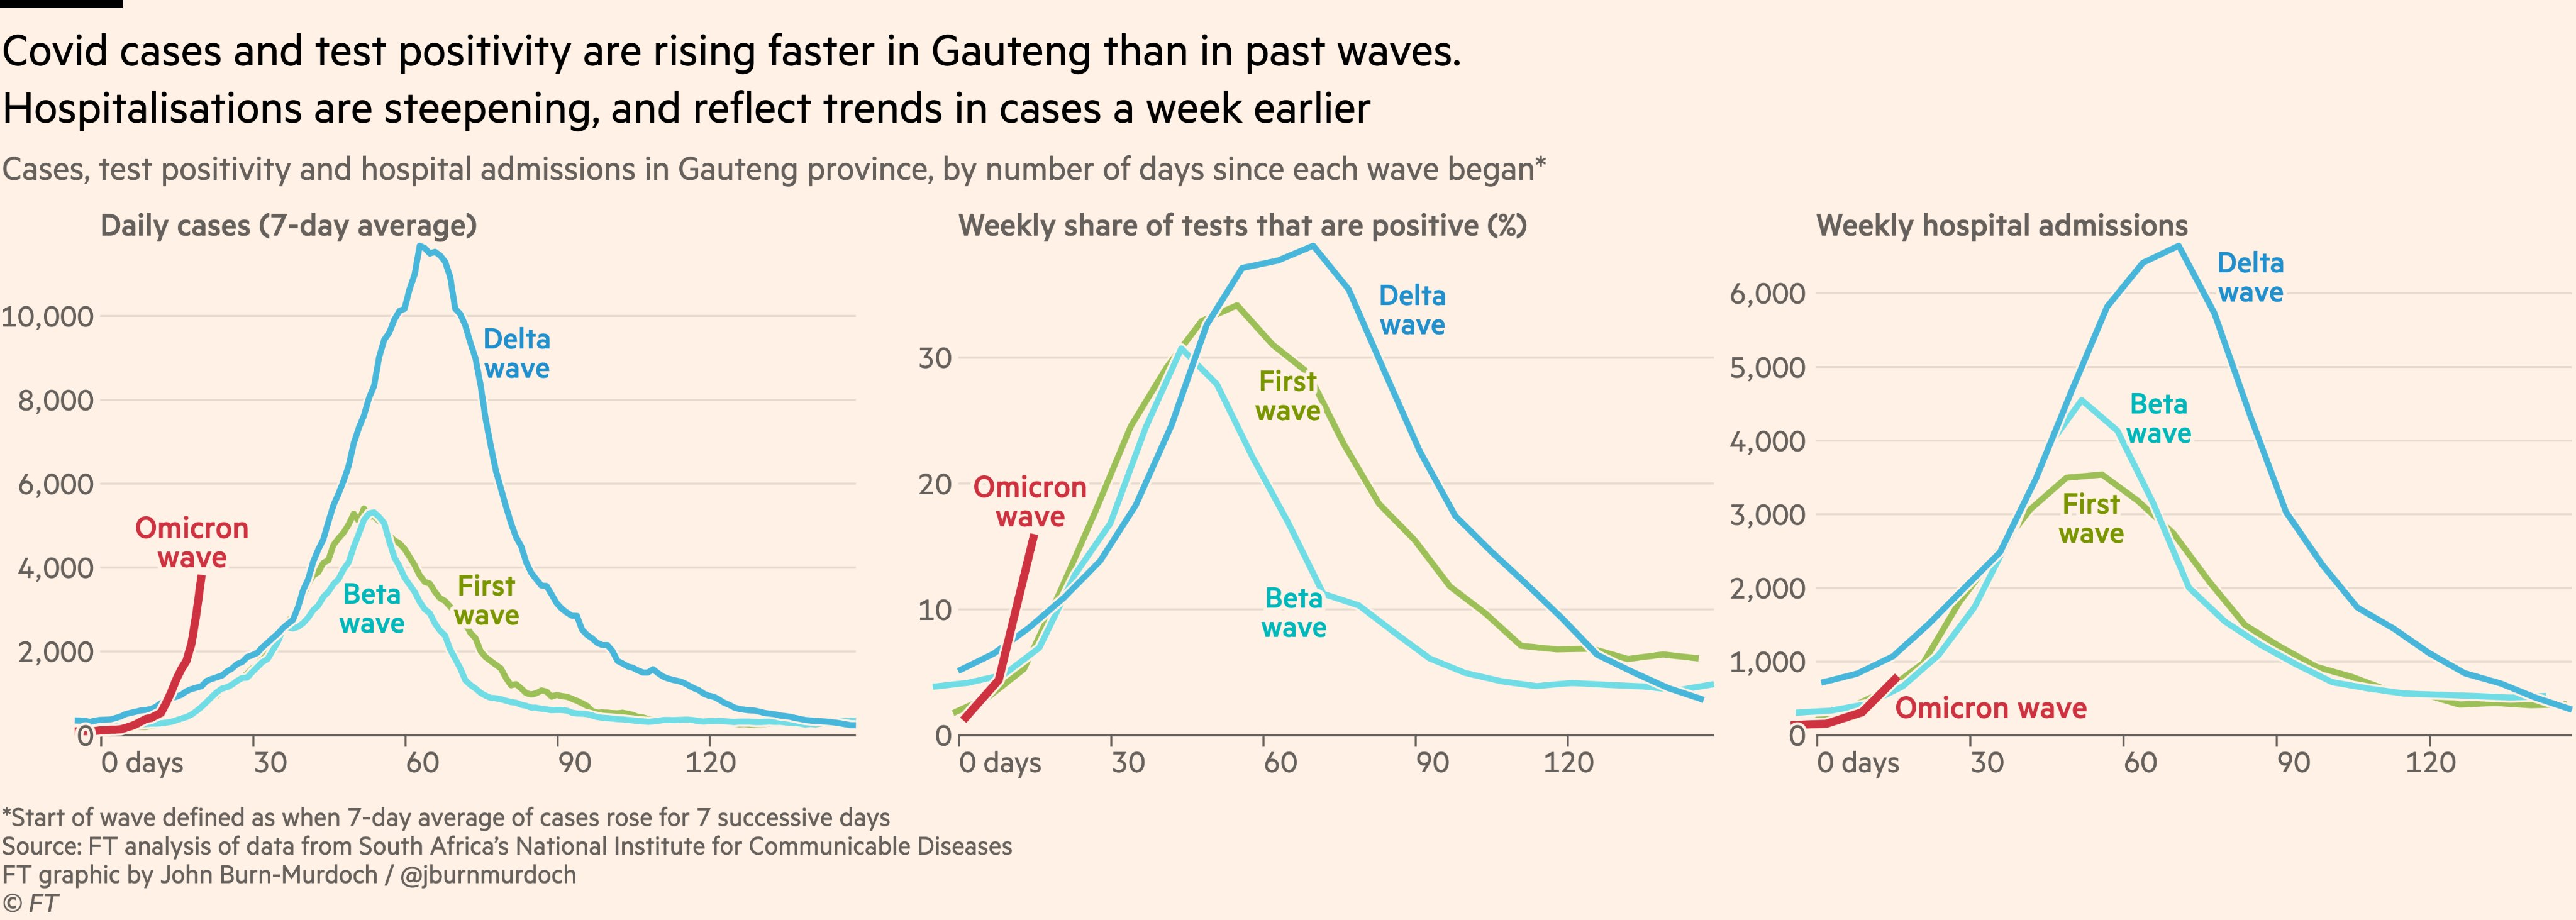
\includegraphics[width=\linewidth]{ft-waves-linear}
\caption{COVID Cases, positivity rate, and hospital admissions from South Africa's Gauteng province, on a log scale (top) and linear scale (bottom). Successive waves are overlaid, showing that the increase in cases due to the Omicron variant was sharper than any previously measured increase, while hospitalizations were much more comparable to previous waves \citep{burn-murdoch_new_2021-1}.}
\label{fig:ft-waves}
\end{figure}

While traditionally, time series information has been limited to charts with time on a linear x-axis, many charts manipulated time to highlight different aspects of the pandemic. In some cases, these modifications provided large amounts of utility for a relatively small increase in complexity; for example, John Burn-Murdoch's decision to index Financial Times COVID graphs to the days since the $N$th case or death. This decision is a small modification of the basic time series plot, but has important consequences in the chart's readability as well as the visual emphasis for users: the graphs in the Financial Times were designed to emphasize "... that there's an inevitability about how coronavirus spreads... even if there are only a few cases in your country today, based on all the data we have, you will end up going along that path, the same path that the likes of Italy and Spain have been on so tragically."\citep{hannenCoronavirusTrajectoryTracker2020a} By placing all countries on an even footing divorced from the temporal randomness of when the first case appeared, the viewer can effectively compare the effect of government policies and other interventions on the trajectory over time\citep{burn-murdochAllCountriesDeath2020,burn-murdochLatestCaseTrajectories2020}. 


The New York Times intentionally violated typical design guidelines in a controversial chart; the x-axis was wrapped around an Archimedean spiral to provide a sense of periodicity in the year-by-year evolution of case counts, as shown in \Cref{fig:nyt-spiral}. The original form of this chart is prone to the line-width illusion \citep{vanderplasSignsSineIllusion2015}, in addition to the well-known problems with polar charts \citep{hofmannGraphicalTestsPower2012,waldnerComparisonRadialLinear2020}. A re-envisioned version created by Sourya Shrestha, aligns counts on the outside of the spiral, and displays them as radial lines, mitigating some of the issues with the line-width illusion by directly showing each line as its own entity, facilitating direct comparisons. 

In addition, the re-envisioned chart includes a reference line at 100K cases/day, which allows the reader to compare the severity of different waves directly. Still, it is more work to interpret and compare peaks on this chart than on a similar linear time series chart with the same data, as the reader must assess line width and then do a mental rotation and shift operation in order to compare with any other time period. By design, this type of chart devotes less area to previous years of the pandemic, which may decrease the amount of focus given to that data.%; whether this is an advantage or disadvantage depends on your perspective and goals when using the chart.

\begin{figure}\centering
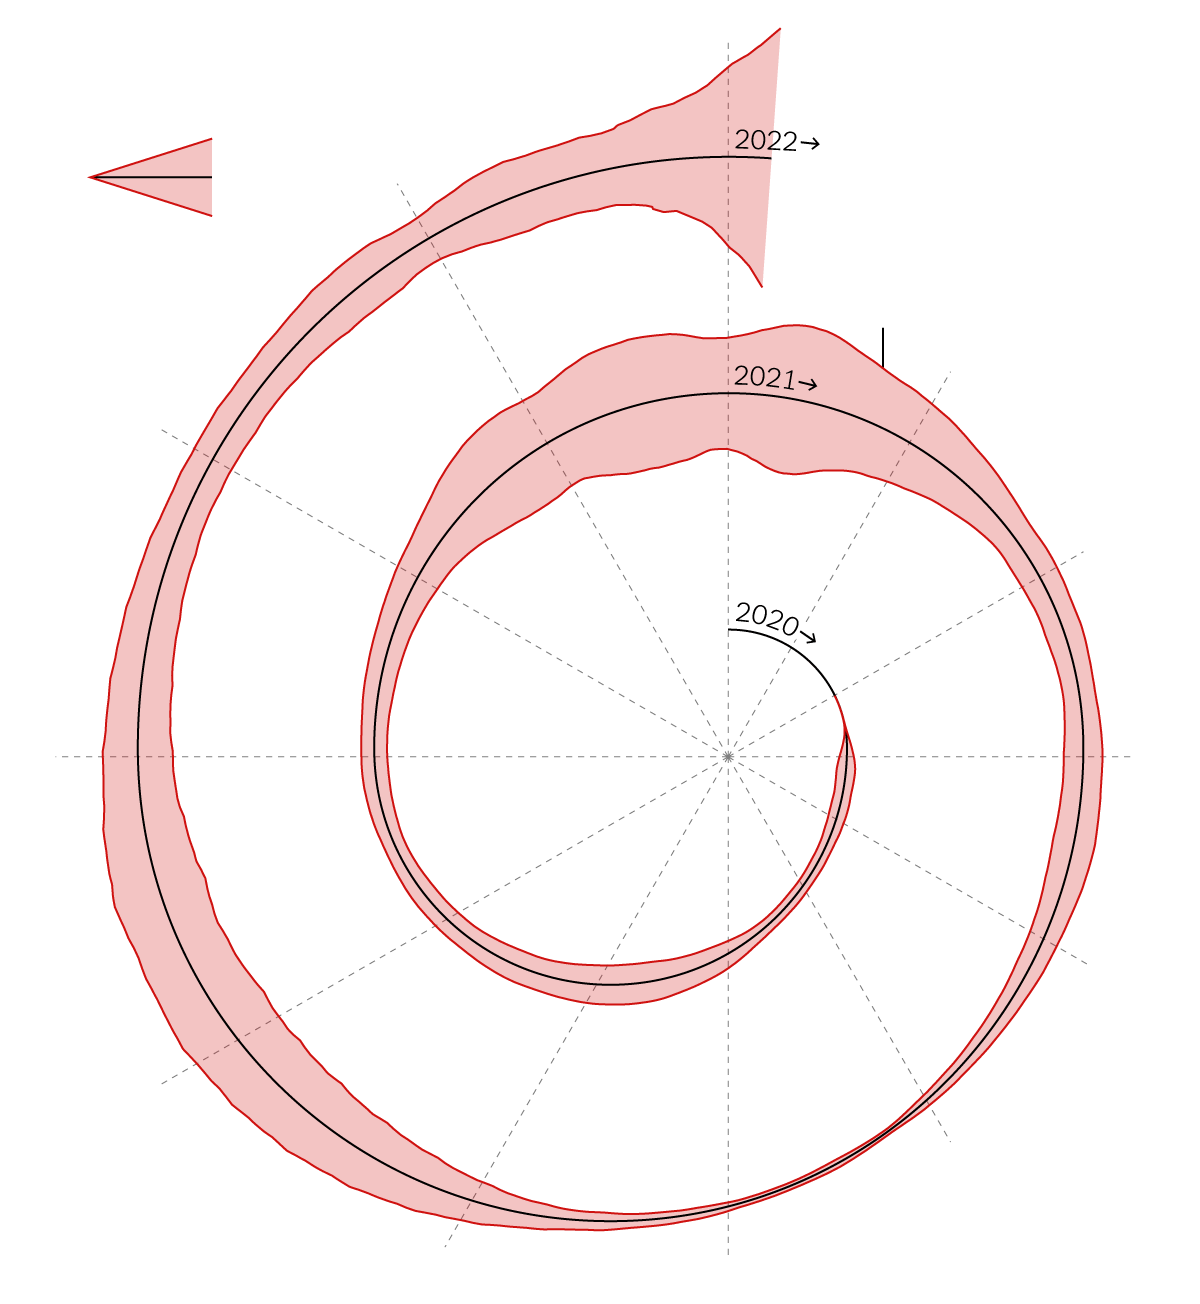
\includegraphics[width=.45\linewidth]{nyt-spiral}\hfill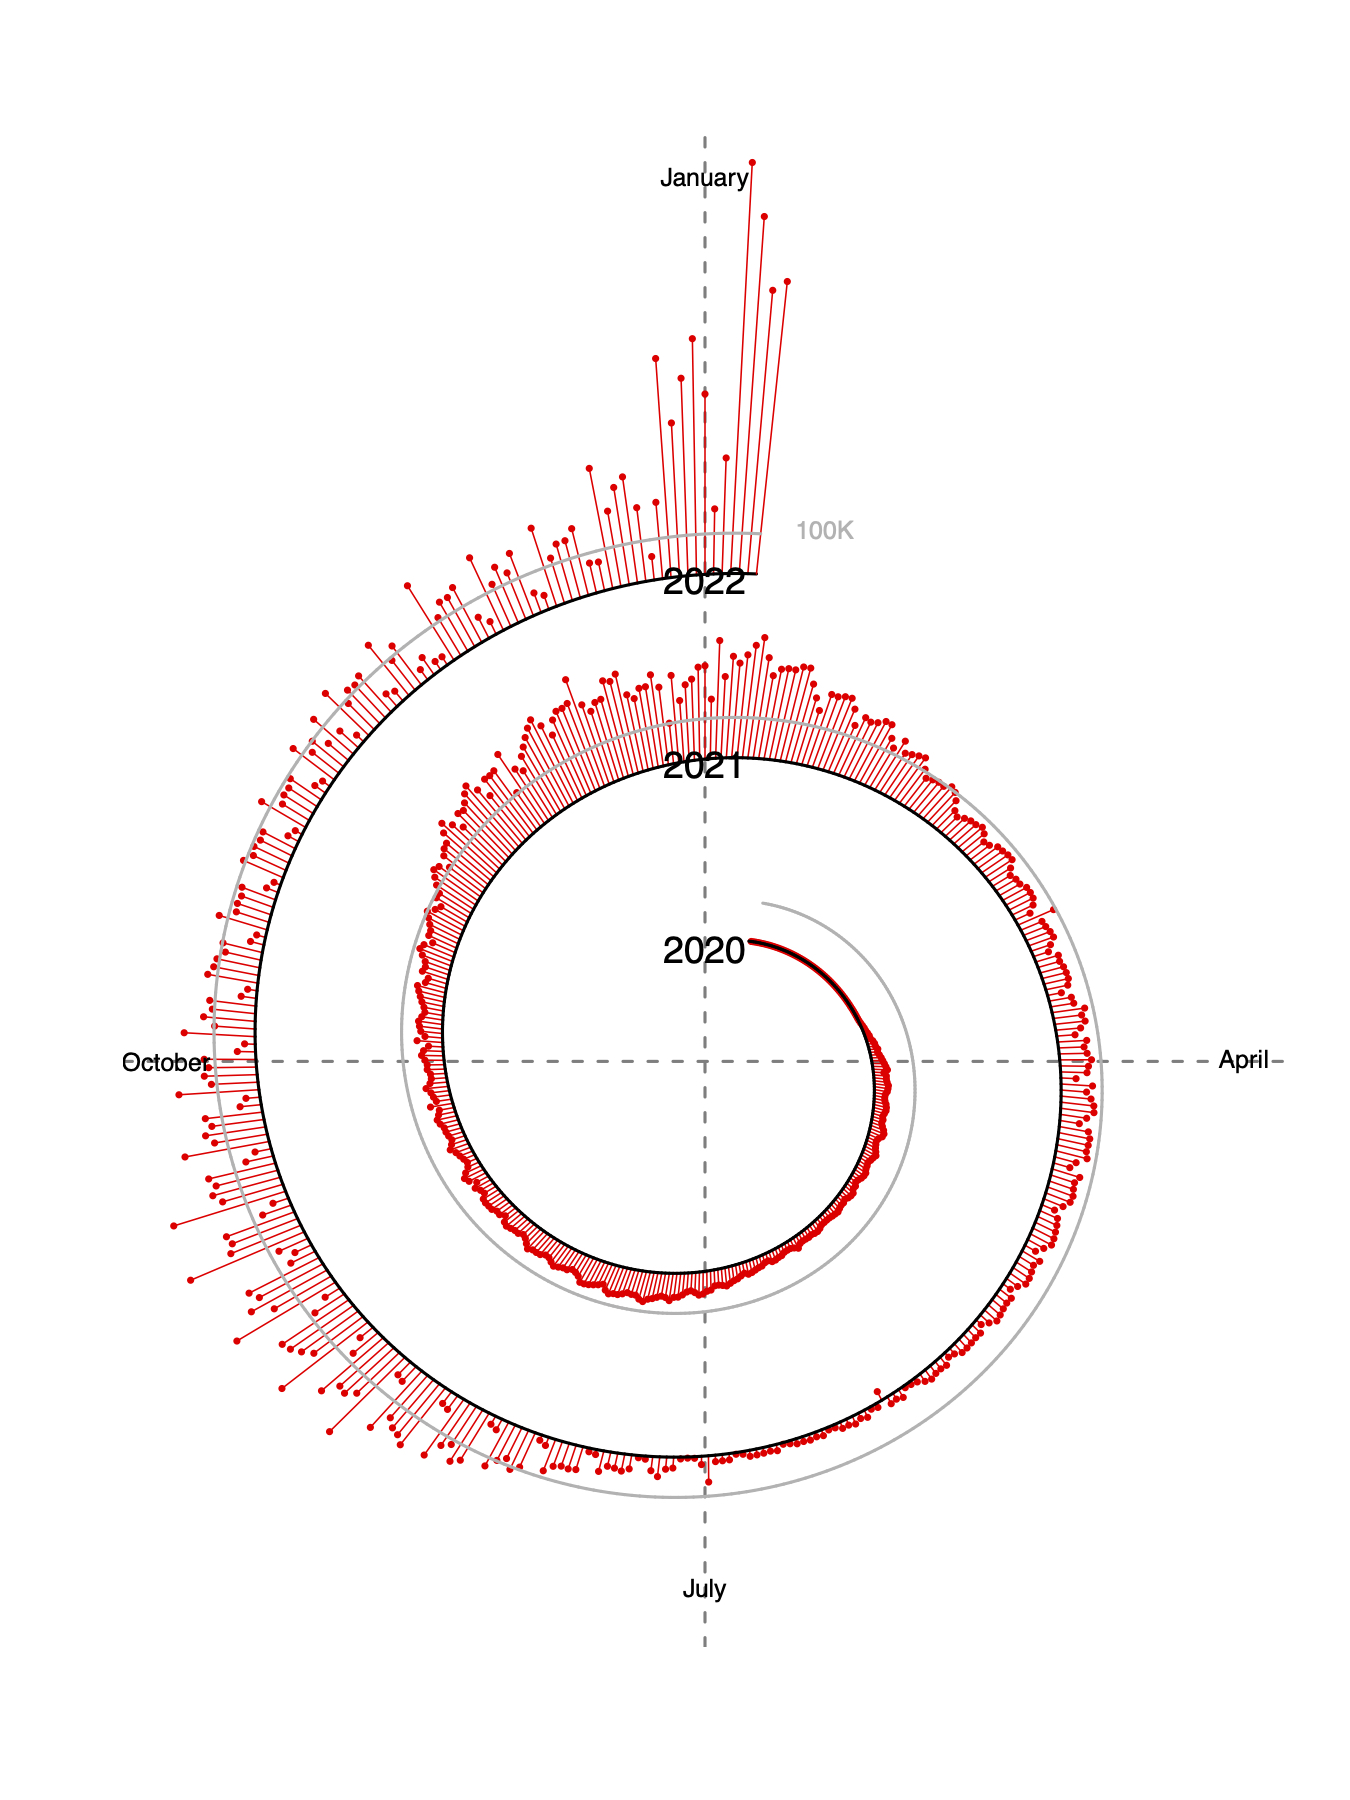
\includegraphics[width=.45\linewidth]{spiral-rework}
\caption{COVID cases in the United States, 2020-2022. The original graph from the New York Times is on the left \citep{shamanOpinionHereWhen2022}, and a reenvisioned version which is more perceptually friendly is on the right \citep{shresthaCovidSpiral2022}.}
\label{fig:nyt-spiral}
\end{figure}

Other designers used the capabilities of web graphics to show the time component in the data through animation. In some cases, this took the form of animated bubble plots XXX add XXX, while others dispensed with the traditional form of a line graph altogether, showing rising case counts using a "bar chart race"; an animated series of bar charts over time that show how case counts in each country are increasing. A typical example can be found on YouTube\citep{clockCoronavirusCasesBar2022}; a screenshot is shown in \Cref{fig:barchart-race}. This type of chart is effective in showing instantaneous changes in counts over days for countries with an extremely high number of cases, but may make it difficult for the viewer to process how cases are changing in countries that do not dominate case counts. By focusing viewer attention on changes in relative totals of case counts, the graphic tends to hide steady, proportional increases in cases across the globe, making it somewhat difficult to perceive large global trends relative to small changes in comparative case counts. 

\begin{figure}
\centering
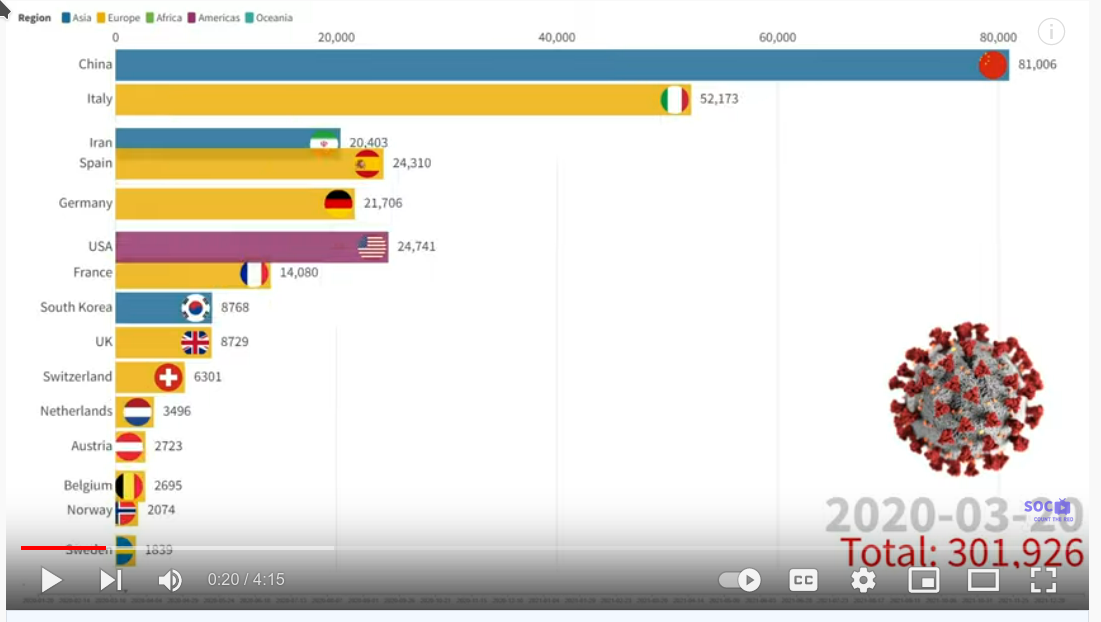
\includegraphics[width=.8\linewidth]{Figures_Web/Bar-chart-race-screenshot}
\caption{A screenshot from Stats on Clock's bar chart race showing counts of COVID cases over time throughout the pandemic \citep{clockCoronavirusCasesBar2022}.}\label{fig:barchart-race}
\end{figure}

As people grappled with the scale of the pandemic and the lives lost as a result, a different set of data displays attempted to provide context to this loss over time. In the New York times, this took the form of a story showing the accumulation of the first 100,000 deaths due to COVID in the US, with occasional short quotes from individuals' obituaries to humanize the names\citep{barryRemembering1000002020}. While this is not a typical time series chart, as the user scrolled through the page the pace of the names increases, showing the scale of the pandemic in a visceral way. A less sentimental dot-density timeline by the New York Times about 9 months later chronicled the nation reaching 450,000 deaths; the difference between the two visualisations brings to mind the quote oft attributed to Stalin: "One death is a tragedy; a million deaths is a statistic" \citep{investigatorSingleDeathTragedy2016}.

A slightly different approach by the BBC's Visual and Data Journalism team, shown in \Cref{fig:bbc-flower}, displayed the COVID cases and deaths as a growing flower, with the stem proportional to the number of cases and the flower petals showing the deaths over time\citep{thebbcvisualanddatajournalismteamCoronavirusHowCan2020}. The visualisation comes with sound as well, an attempt to make the pandemic an auditory experience as well as a visual one. The form, animation, and auditory experience are all indicative of an emotional appeal \citep{kostelnick_re-emergence_2016,dignazio_data_2020}; with the flower representation as an explicitly recognized symbol of grief; it is clearly not about showing specific case counts and deaths numerically.

\begin{figure}
\centering
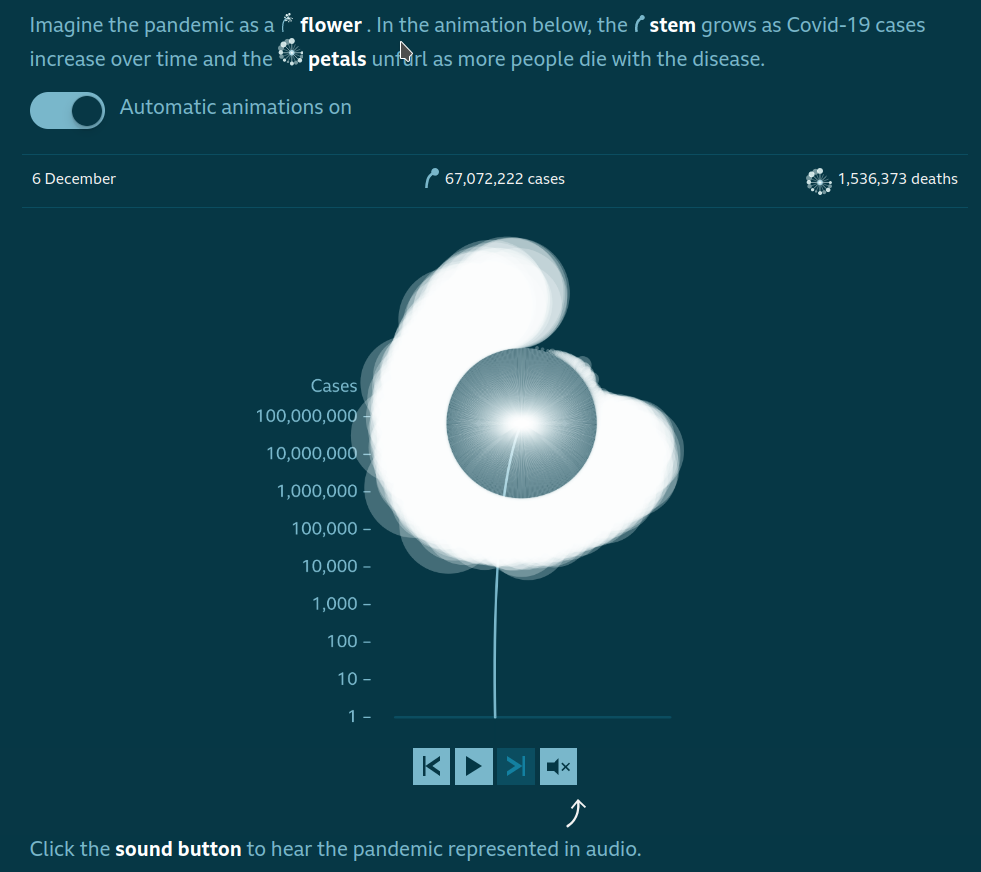
\includegraphics[width=.8\linewidth]{Figures_Web/BBC_flower_time_series}
\caption{The BBC Visual and Data Journalism Team's COVID flower, showing the cases and deaths over time \citep{thebbcvisualanddatajournalismteamCoronavirusHowCan2020}.}\label{fig:bbc-flower}
\end{figure}
% BBC flowers w/ sonification https://www.bbc.co.uk/news/resources/idt-7464500a-6368-4029-aa41-ab94e0ee09fb

% Other animations?

\section{The ranking narrative}
\label{sec:rankings}

"The plague is always the others." This is the short formula for dealing with infectious diseases from a historical perspective \citep{thiessen2021}. Closing the borders and restricting access to the country became a popular means of controlling the spread of the disease at several different points during the pandemic. Unsurprisingly, the prevailing visual narrative focused on comparisons often fueled by political rivalry, historical dependencies, recent withdrawal from supranational institutions or regional competitions. An ongoing debate about the true extent of the dangers of COVID-19 and how best to combat it, combined with daily availability and public access to data across administrative levels, fostered ongoing competition and the use of leaderboards to show how bad case counts were somewhere else. 

\begin{figure}\centering
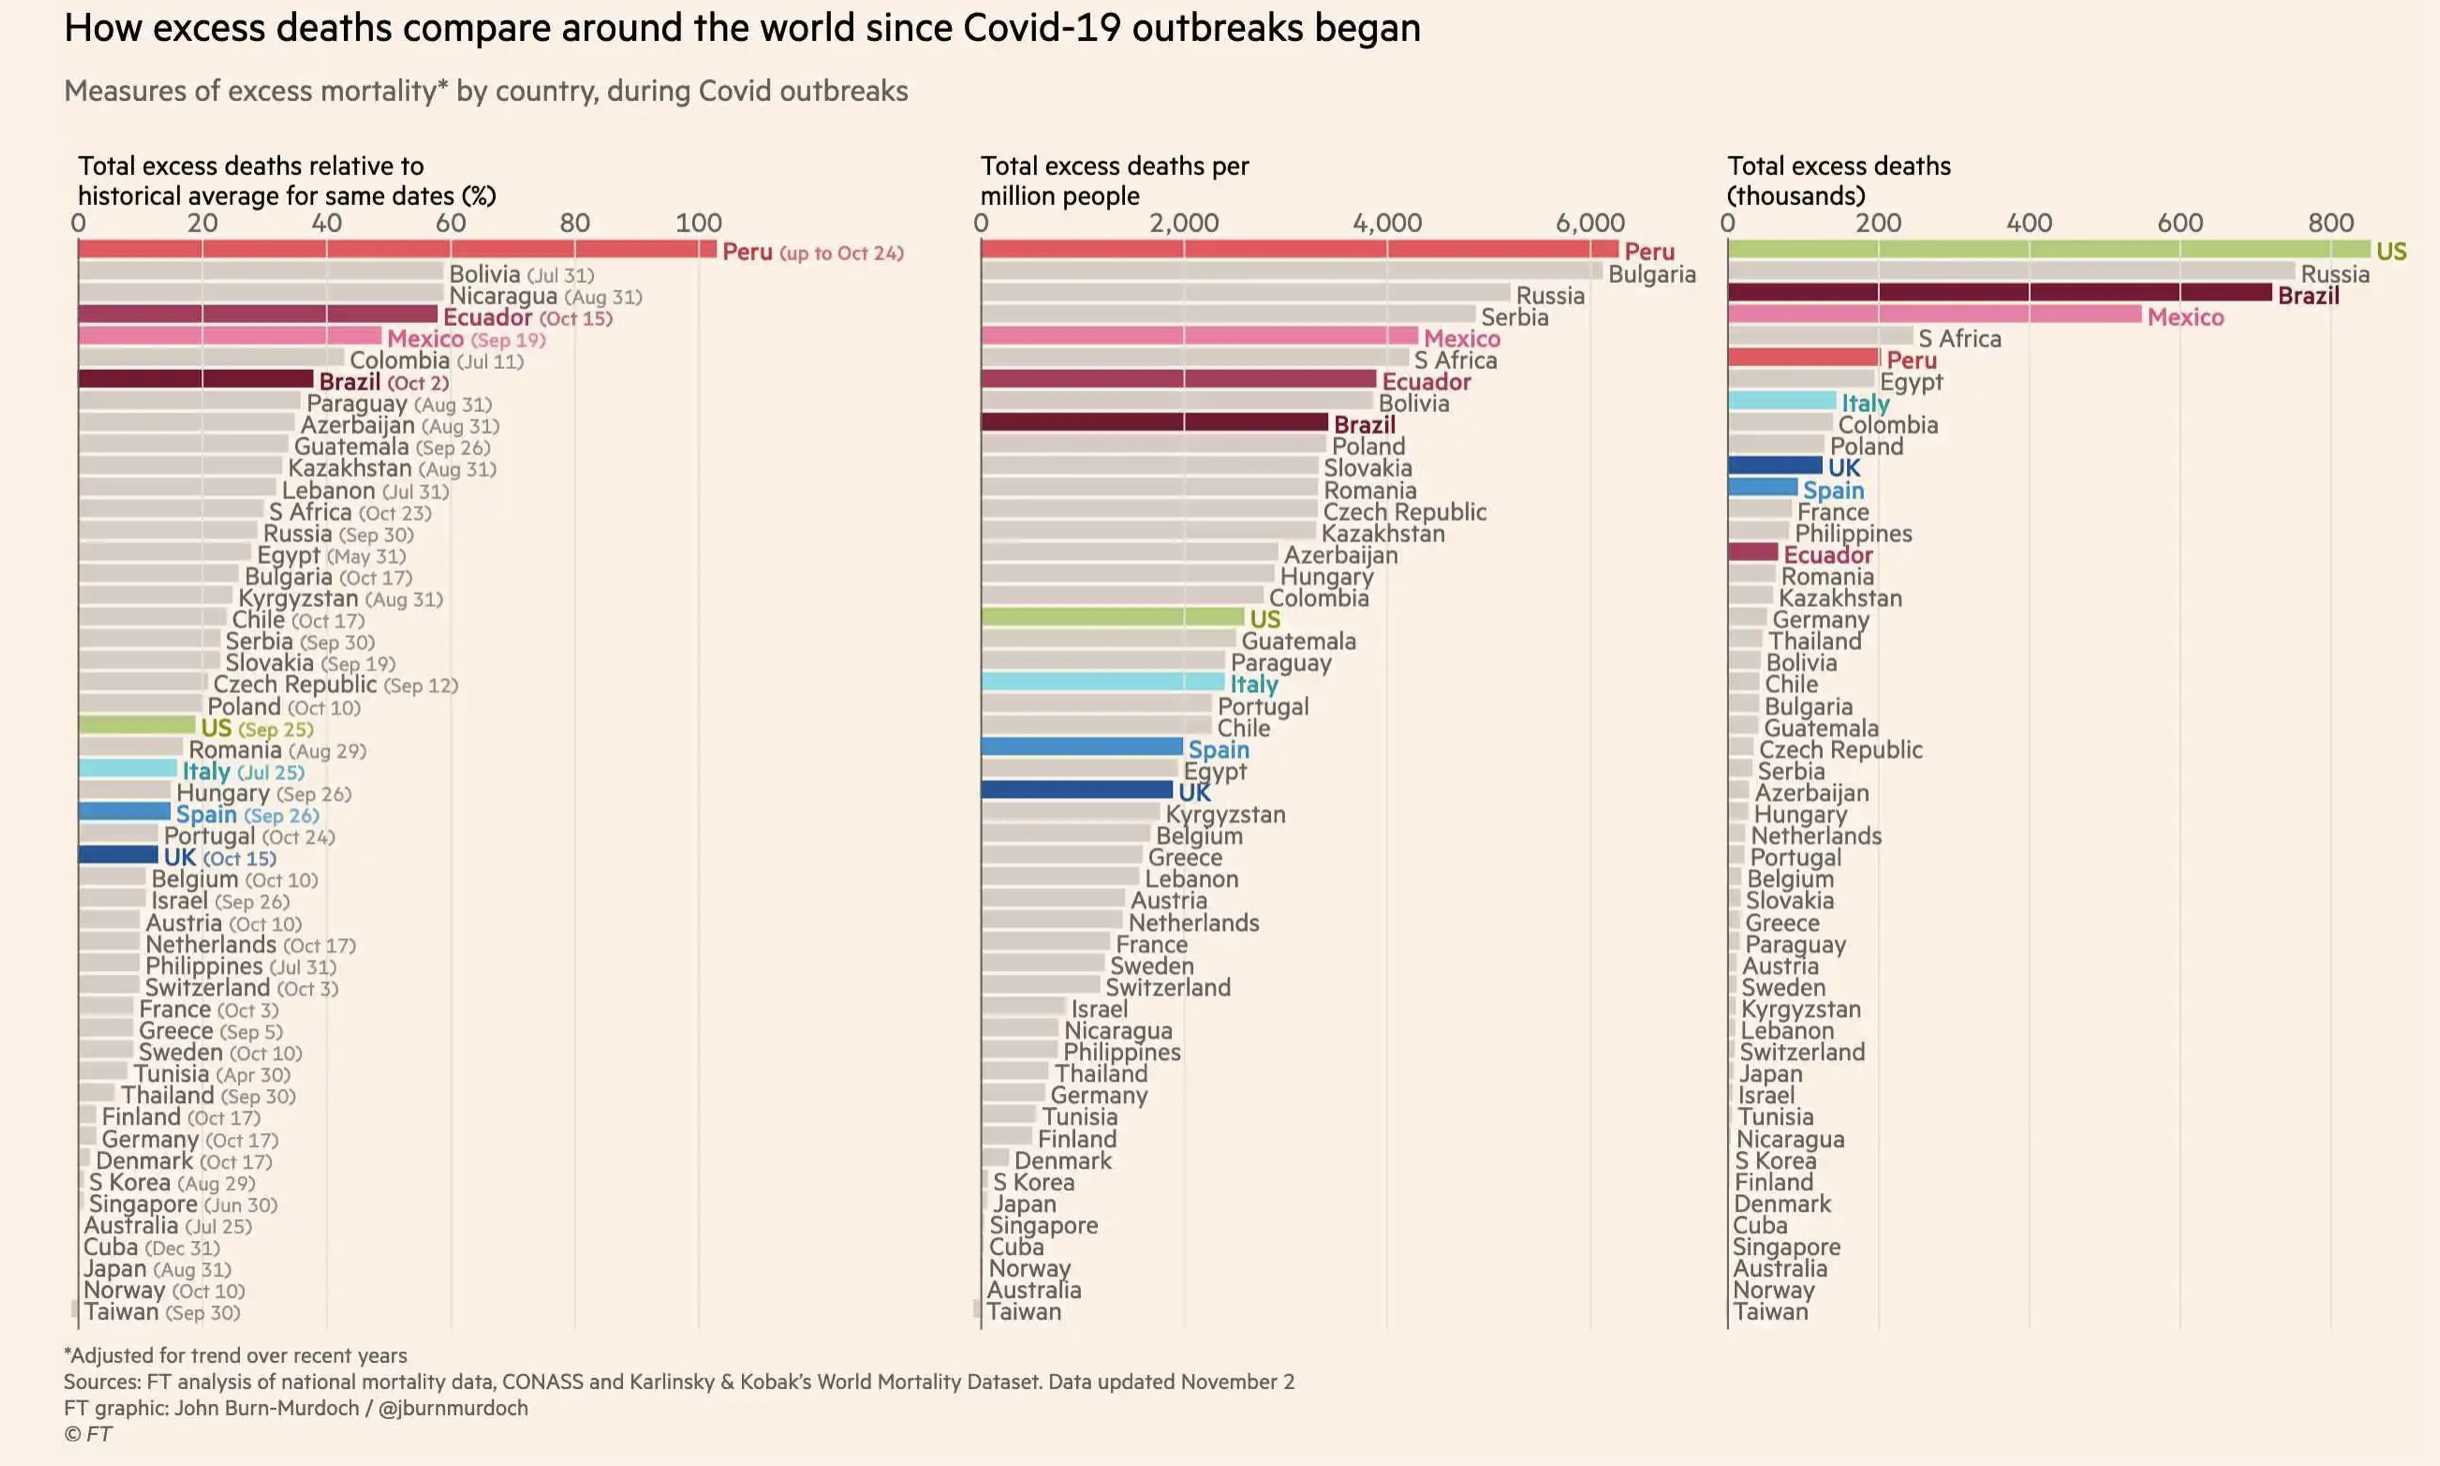
\includegraphics[width=\linewidth]{Figures_Web/ft_deathrates_bar}\\
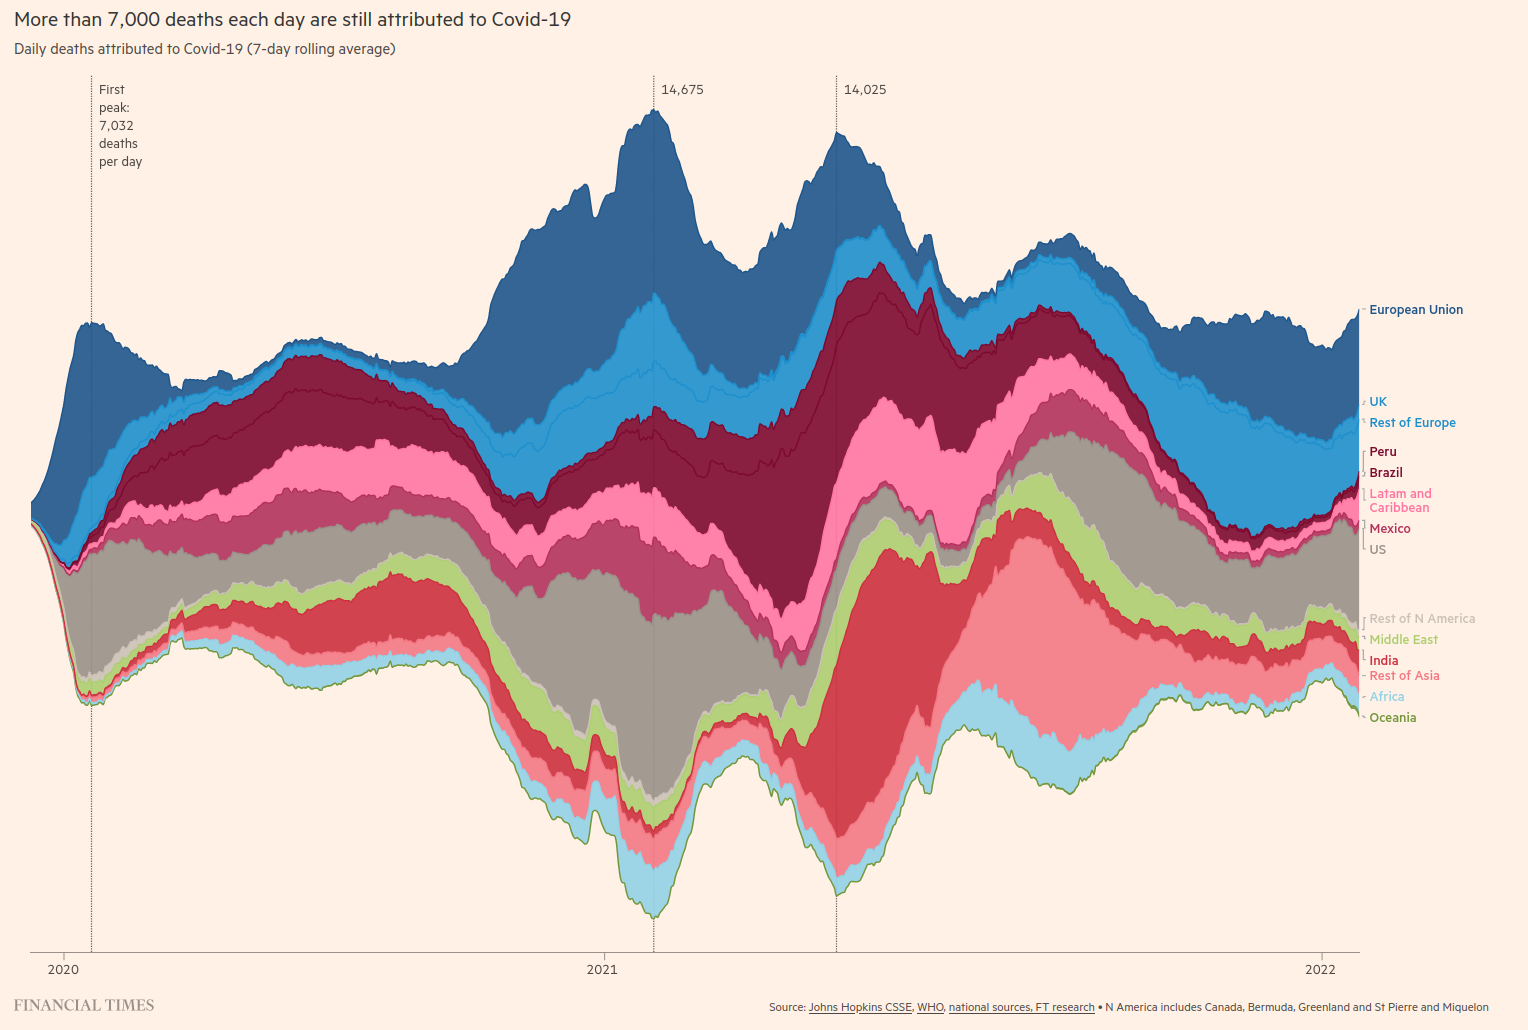
\includegraphics[width=\linewidth]{Figures_Web/ft_deathcounts_area}
\caption{Ordered death rates in countries and the temporal evolution of the death toll share in major world regions \citep{CoronavirusTrackerLatest2021}.}
\label{fig:ft-death-ranking}
\end{figure}

The bar charts used for this purpose (see top image in \Cref{fig:ft-death-ranking}) are straightforward and provide a good way to show the ``leading'' countries or regions. Emphasis on specific countries is either preconfigured by the creator of the chart or can be modified interactively in the online version by check boxes and drop-down menus. These bar charts also allow easy adjustment of the count data to population size or other meaningful standard. Streamgraphs (see lower image in \Cref{fig:ft-death-ranking}) are a special type of stacked area graphs and became quite popular around 2008 when they were used by the New York Times to visualise box office results of movies \citep{streamgraph}. Their usefulness depends heavily on the clarity of the pattern, as well as design choices such as the ordering of the different groups. Small variations in the proportions of the groups are almost impossible to detect, but streamgraphs give a good indication of which group is predominant at any given time, even though they are subject to the line-width or sine illusion \citep{vanderplasSignsSineIllusion2015}. When paired with the bar charts showing excess mortality, the streamgraph provides temporal context to the instantaneous information in the bar graph.

Often, these comparative charts were combined with policy discussions, with individuals challenged to spot certain policy interventions on the case-count graphs of different localities with different policies\citep{weissThese12Graphs2020}. \Cref{fig:policy-comparison} shows a chart from an article which appeared in The Federalist, a conservative outlet in the United States, suggesting that mask mandates are ineffective because it is difficult to spot the impact of the mask mandate on the overall trend of cases. Of course, mask mandates are but one component of a much broader pandemic management strategy, but the goal of the chart is clear; the reader is supposed to conclude that cases and masks are not associated. These charts were so common on social media that media outlets ran stories identifying them as misinformation \citep{reutersstaffFactCheckMask2020}; clearly, comparative charts were effectively deployed to misinform as well as to inform.

\begin{figure}
\centering
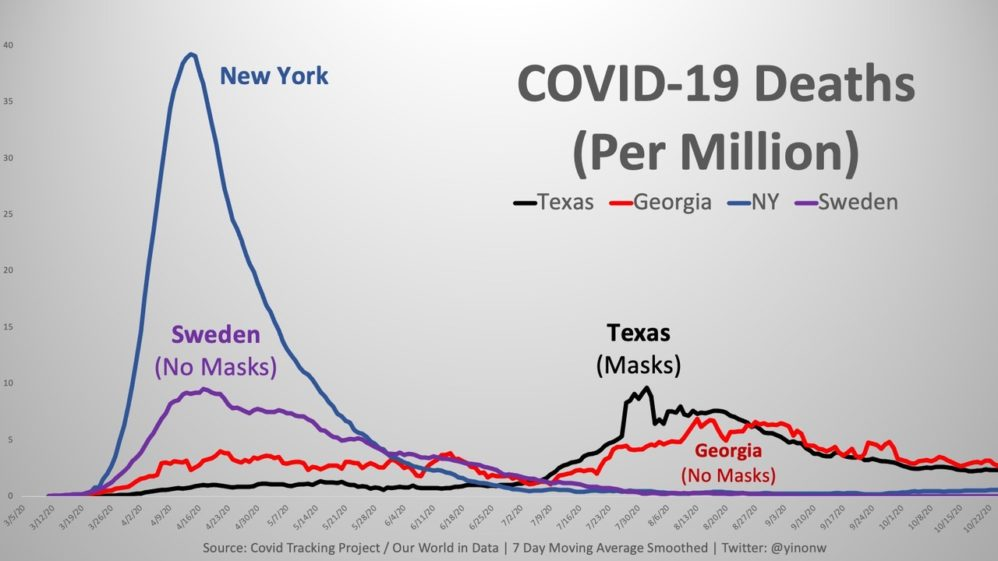
\includegraphics[width=.8\linewidth]{Figures_Web/Deaths-NY-TX-GA-Sweden-Federalist.jpeg}
\caption{Deaths per million people in New York, Sweden, Texas, and Georgia, as shown in the Federalist \citep{weissThese12Graphs2020}. The goal of this comparison chart is to lead the reader to conclude that masks are ineffective, as there is not a clear difference between Texas and Georgia. New York is also shown (though not labeled as requiring or not requiring masks), and Sweden is shown as well, despite not being a US state at all, leading the critical reader to conclude that the time series shown in this chart have been cherry-picked to make a rhetorical point.}\label{fig:policy-comparison}
\end{figure}



\section{To log or not to log}\label{sec:logs}
As COVID cases grow quasi-exponentially while there are susceptible members of the population (subject to the effectiveness of mitigation measures and testing availability), it seems natural to use log scales to allow for more effective comparisons of slight changes in case counts over time. In addition, log scales make it possible to compare regions with different populations or infection rates in the same chart. As noted previously, however, interpreting log scales requires levels of numerical sophistication that may not be appropriate for the general public. Even researchers do not always read and interpret log scales correctly\citep{mengeLogarithmicScalesEcological2018}; expecting the general public to do so is difficult under normal circumstances\citep{hecklerStudentAccuracyReading2013} is difficult. When panic, fear, uncertainty, and doubt about the situation are added to the mix, it is easy to imagine that we become even worse when interpreting graphics.
% Discussion of how this section's conclusions change with the pandemic

One issue with assessing the use of log scales is that their effectiveness changes with the stage of the pandemic and the amount and variety of data shown. Initially, log scales were incredibly useful at showing case counts, because minimal mitigation measures were in place and the growth of case counts (or presumptive positive cases, in absence of available testing) was fairly close to exponential. In addition, the use of log scales allowed for the comparison of total cases across entities with large population differences; in the US, we could compare cases in New York and California with cases in Michigan and Washington, even though the populations (and corresponding case counts) of Michigan and Washington are much lower than the populations (and case counts) of either New York or California. 

\begin{knitrout}\footnotesize
\definecolor{shadecolor}{rgb}{0.961, 0.961, 0.961}\color{fgcolor}\begin{figure}

{\centering 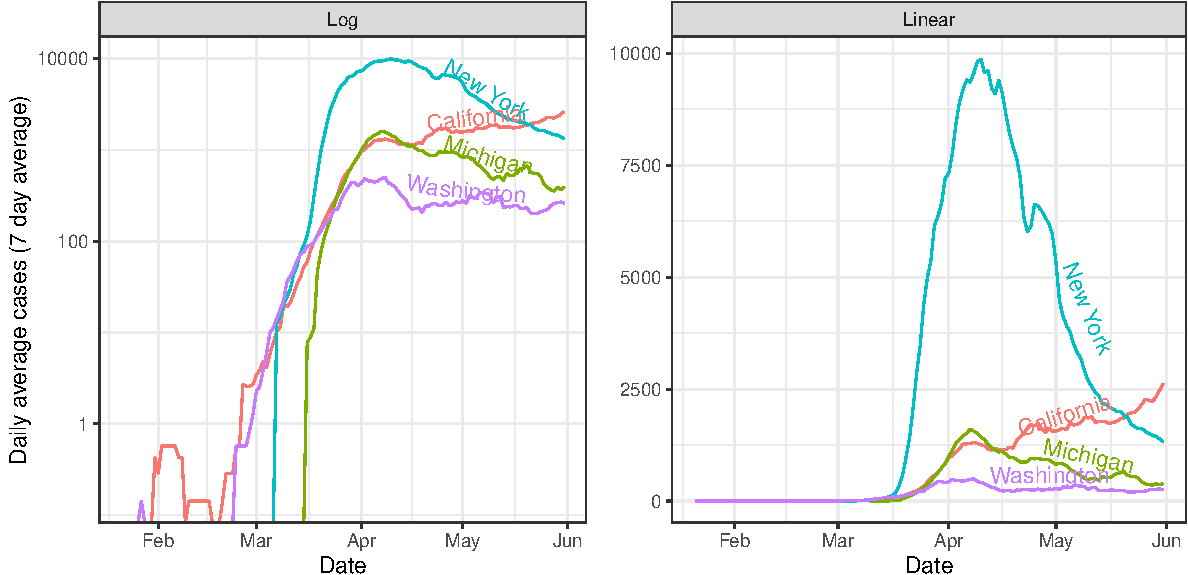
\includegraphics[width=\linewidth]{Figures_R/fig-log-scale-initial-1} 

}

\caption[In the early stages of the pandemic, log scales allowed the comparison of raw case counts in locations with vastly different population and case counts]{In the early stages of the pandemic, log scales allowed the comparison of raw case counts in locations with vastly different population and case counts.}\label{fig:log-scale-initial}
\end{figure}

\end{knitrout}

While log scales are not necessarily intuitive, many outlets tried to make the graphs more intuitive by adding reference lines, as shown in \Cref{fig:diag-ref-lines}. 

\begin{figure}
\centering
\includegraphics[width=.8\linewidth]{ft-COVID-19-deaths}
\caption{Reference lines to compare exponential growth rates of deaths in different countries. This provides some additional context that may help individuals use log scale data more successfully. This approach was first featured in the Financial Times, but was quickly adopted by the New York Times, 91-DIVOC, and other outlets. Graph from the Financial Times (March 23, 2020), image from \citet{kosaraPraiseDiagonalReference2020}.}
\label{fig:diag-ref-lines}
\end{figure}

% Problems with log scales
However, after the first wave of COVID, the issues with log scales became more apparent; it was difficult to detect slight increases in case counts that indicated the beginning of a new wave amid a background level of spread, as demonstrated in  \Cref{fig:log-scale-failures}. Diagonal reference lines from the origin were also less helpful, as the growth of cases or deaths was no longer approximately exponential and varied over time; for these reference lines to be effective there would need to be a clear idea of when the case counts started to increase exponentially, which is difficult to determine whilst in the thick of a potential COVID wave. Occasionally graphs with manually drawn reference lines were made available, but usually only in a retrospective manner, as in \Cref{fig:log-scale-ref-multiple}. 

\begin{knitrout}\footnotesize
\definecolor{shadecolor}{rgb}{0.961, 0.961, 0.961}\color{fgcolor}\begin{figure}

{\centering 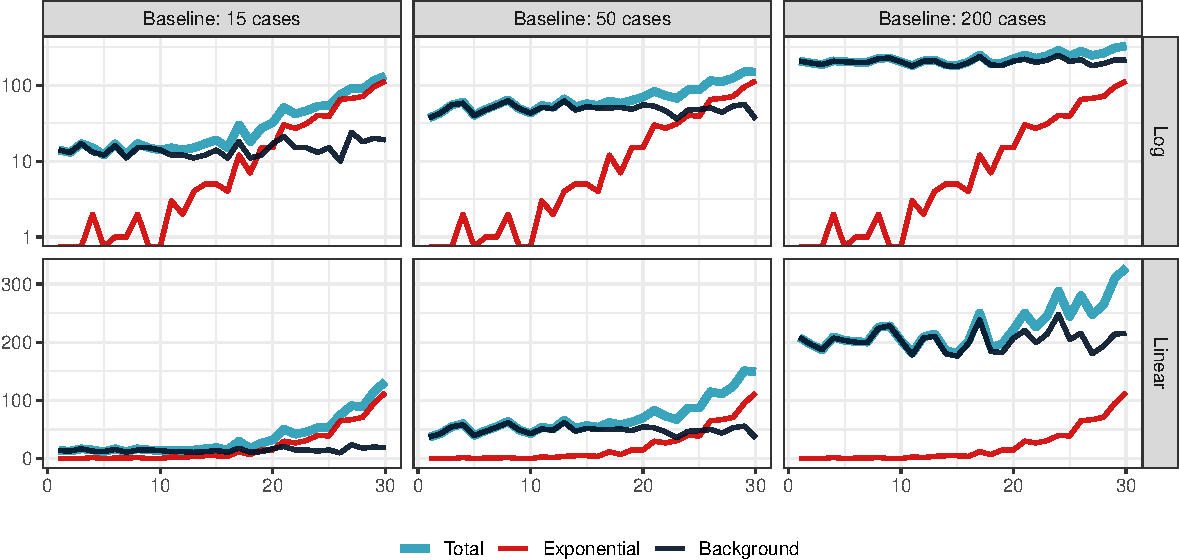
\includegraphics[width=.95\linewidth]{Figures_R/fig-log-scale-failures-1} 

}

\caption[One problem with log scales is that if there is a background level of spread, it can be hard to notice the introduction of an additional source of exponential spread]{One problem with log scales is that if there is a background level of spread, it can be hard to notice the introduction of an additional source of exponential spread. Linear scales do not have this problem - the exponential source is noticeable very quickly in the total line, but on the log scale it is much harder to discern when the exponential source causes the total line to diverge from the background. In the top-right corner, it is difficult to identify that there is an exponential increase in cases amid the baseline of a uniform level of spread over time, even though the exponential source makes up approximately 50\% of the cases at the end of the time period shown.}\label{fig:log-scale-failures}
\end{figure}

\end{knitrout}

% Focus primarily on time-series graphs (as opposed to log scales in colour)

\begin{figure}
\centering
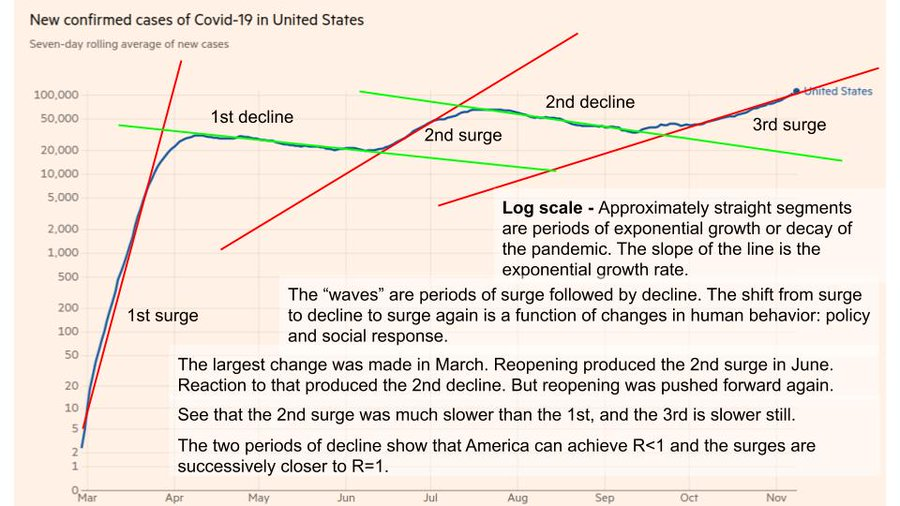
\includegraphics[width=.8\linewidth]{ft-reference-lines}
\caption{An annotated time series from the Financial Times which appeared on Twitter on November 12, 2020. This chart has annotations which show the decreasing $R_{eff}$, the effective rate of exponential spread, in successive peaks of the pandemic, with periods of $R_{eff}<1$ between surges in cases. These annotations assist the reader with drawing complex conclusions from the chart, but are difficult to automate and thus tend to be manually curated \citep{gubrudDrEricDingWeVe2020}.}
\label{fig:log-scale-ref-multiple}
\end{figure}


% Problems with linear scales
While log scales have their problems, linear scales are not immune from issues either. It can be very difficult to adequately compare to past situations when looking at the full time series of case counts. For example, in \Cref{fig:linear-scales-ref-lines}, it is difficult to tell whether the first wave of COVID cases in March 2020 had an increase as fast as that in January of 2021; it is even more difficult to compare the order-of-magnitude of change in case rate growth of January 2021 relative to January 2022 when the more contagious omicron variant became prevalent. 

\begin{knitrout}\footnotesize
\definecolor{shadecolor}{rgb}{0.961, 0.961, 0.961}\color{fgcolor}\begin{figure}

{\centering 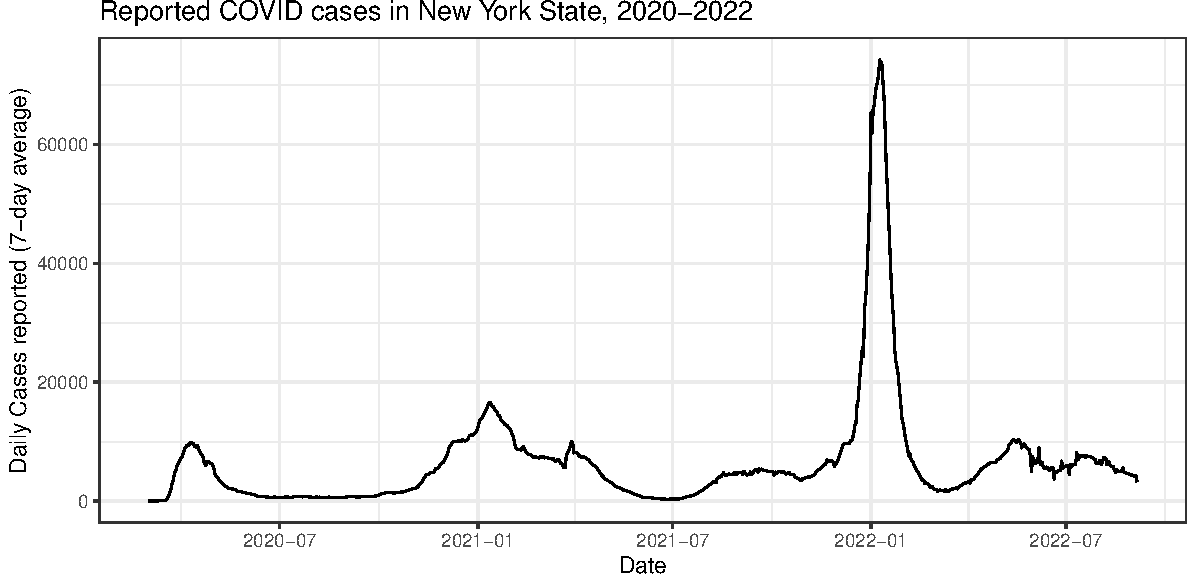
\includegraphics[width=.8\linewidth]{Figures_R/fig-linear-scales-ref-lines-1} 

}

\caption[Reported COVID cases in New York State, 2020-2022]{Reported COVID cases in New York State, 2020-2022. The linear scale makes it difficult to compare the trajectory of different waves to determine how severe the current status is relative to the past, because the primary contrast is the height of the relative peaks, rather than the growth \emph{rate}. A similar graph on the log scale would have the peaks at much more similar heights (though there would still be a difference), allowing the reader to focus on other information, such as the slope of the relative lines.}\label{fig:linear-scales-ref-lines}
\end{figure}

\end{knitrout}


% Discussion of sites which allow the user to switch back and forth between scales

It is not clear that the use of log or linear scales during the COVID-19 pandemic had a large effect on public opinion. Several studies were conducted in the early stages of the pandemic \citep{romanoScaleCOVID19Graphs2020, seviLogarithmicLinearVisualizations2020, ryanGraphsLogarithmicAxes2020} and results seem to suggest that while individuals have difficulty understanding log scale graphs, these issues do not tend to affect their support for intervention measures, perhaps in part because COVID-related news saturated the news and opinions were set outside of information provided in the experiments. This saturation makes it difficult to study the graphical influences while removing effects of popular opinion, political leaning, and emotional sentiment relating to the pandemic. 

If we evaluate the use of log and linear scales under the more general context of exponential (or near-exponential) growth rates, however, we can gain some clarity as to their use in this particular context. We are abysmal at forecasting exponential growth, vastly under-estimating future growth by using linear or quadratic approximations \citep{wagenaarExtrapolationExponentialTime1978a,lawrenceExploringJudgementalForecasting1992,timmersInverseStatisticsMisperception1977a}. If the goal of a chart of COVID case counts is to allow individuals to forecast the trend and make decisions accordingly, then using a log scale (with all of its pitfalls in understanding) may be the best option, as it at least replaces the need to forecast along an exponential curve with the need to forecast along a straight line. However, it is not clear that individuals can transfer that prediction back to a linear scale. If the goal of presenting a chart of case counts is to tell the story of what has happened (rather than supporting future decision-making), then it is undoubtedly better to present the data on a more familiar linear scale that requires less cognitive load on the part of the viewer. 

Unfortunately, there are not a lot of good options for supporting forecasting decisions in mathematically unsophisticated viewers. Guide lines, like those used in the Financial Times, were helpful in the initial phases of the pandemic, but no outlets that we are aware of shifted the lines to show the growth rate of the current peak (as opposed to the initial peak), and due to the issues shown in \Cref{fig:log-scale-failures}, these guide lines may not have been all that successful in any case. Those hoping to create successful time series charts that allow forecasting are thus left with two options: deal with our inability to forecast exponential growth, or deal with most individuals' inability to translate log scales into practical reality. 


\section{Summary and Discussion} \label{sec:summary}
Throughout the pandemic (thus far), visual representations of data have been an integral part of scientific communication. While not always optimal, these graphics have attempted to provide meaningful context, to encourage individual and collective action, and to help individuals grapple with the scale of the pandemic in cases, deaths, vaccinations, and interventions. As in any developing situation, choices made at some points in the pandemic did not always persist - many news outlets refined their charts and approach to the design of graphics over the course of the pandemic. This evolution of graphical forms has provided us with an opportunity to evaluate what worked and did not -- and why -- in a context of broad general interest. 

The visual narratives of the pandemic which have persisted over time are due in part to the rise of data journalism and interactive graphics platforms which ensure that every outlet has the ability to host engaging and visually appealing graphics; however, while these graphics are nice to look at, not all are equally functional or useful for communication purposes. Thus, analyzing the rich collection of visualisations produced as part of the pandemic provides a unique opportunity to examine how these graphics were (and were not) effective, as well as the design decisions made during their creation. As in any situation, good tools can be used and misused freely; we have seen charts and graphics used to perpetuate misinformation and misleading claims, even though it is far more common for charts and graphs to be used for good - to educate and inform the public.

The COVID 19 pandemic has amply demonstrated that policies are only effectively implemented and followed by the population if they are accepted by a large majority of the population. To achieve this goal, it is essential that scientists, governments, the media, and citizens all effectively communicate in order to justify the appropriateness, usefulness and relevance of the measures. This is as true for guidelines about the use and creation of charts as it is for policies like masks and vaccines. % Making it a bit more explicit

The pandemic and graphics used to show the ebb and flow of COVID cases highlight the challenges of data visualisation in the modern era. Even with numerous guidelines and standards for graphics, it is not straightforward to communicate about complex data, and creating charts which fully represent the intended message or messages is a challenge. It is essential that we continue to study how graphics are perceived and interpreted, supporting the guidelines and standards which exist with user studies that ground these rules in science. 

% Ubiquity of the data, persisting general interest on the topic, the rise of data journalism, and the opportunities provided by interactive and dynamic internet platforms contributed to a an ongoing trend on visual narratives of the COVID-19 pandemic. Graphical displays are used as weapons for information, but also for misinformation. Despite a growing number of guidelines for communicating statistical results transportation of the intended messages is not always straightforward and remains a challenge. The deciphering of visual icons and best practices of visual communication require furhter studies on perception and graphics.

%Broad conclusions: 
% importance of scientific communication
% graphs are weaponized for misinformation as well as information?
% Need to improve broad guidelines for communication, underpinning with studies on perception and graphics that 

%% -- Optional special unnumbered sections -------------------------------------
\newpage
\section*{Computational Details}
Graphics included in this paper not sourced from media outlets were created using data published by the New York Times at \url{https://github.com/nytimes/covid-19-data/}. Graphics were created using ggplot2\citep{ggplot2} and \proglang{R}~4.1.2. \proglang{R} itself and all packages used are available from the Comprehensive \proglang{R} Archive Network (CRAN) at \url{https://CRAN.R-project.org/}.

Archived data and code to create the figures in this paper can be found at \url{https://github.com/srvanderplas/covid-visualization-dssv}.

\section*{Archived Information}
This paper references many news articles which contain interactive graphics. In order to preserve these graphics (which depend on a great many external files), the authors have preserved many of the interactive graphics as self-contained html files \citep{news-file-archive}. 
The authors have also made extensive use of the Internet Wayback Machine, which aims to preserve the state of important web pages as they change over time.

\section*{Acknowledgments}

First ideas have been presented at DSSV 2020. We thank our colleagues, the reviewers, and the editors for valuable feedback and encouragement to complete and revise this manuscript.

%% -- Bibliography -------------------------------------------------------------
%% - References need to be provided in a .bib BibTeX database.
%% - All references should be made with \cite, \citet, \citep, \citealp etc.
%%   (and never hard-coded). See the FAQ for details.
%% - JSS-specific markup (\proglang, \pkg, \code) should be used in the .bib.
%% - Titles in the .bib should be in title case.
%% - DOIs should be included where available.

\bibliography{refs}


%% -- Appendix (if any) --------------------------------------------------------
%% - After the bibliography with page break.
%% - With proper section titles and _not_ just "Appendix".
% 
% \newpage
% 
% \begin{appendix}
% 
% \section{More Technical Details} \label{app:technical}
% 
% 
% Appendices can be included after the bibliography (with a page break). Each section within the appendix should have a proper section title (rather than just \emph{Appendix}).

%For more technical style details, please check out JSS's style FAQ at
%\url{https://www.jstatsoft.org/pages/view/style#frequently-asked-questions}
%which includes the following topics:
%\begin{itemize}
%  \item All main words in titles and headers start with a capital.
%  \item Use vectorized graphics formats such as eps and pdf when possible. Graphics should be of high quality while trying to minimize the file size.
%\end{itemize}

% 
% \section[Using BibTeX]{Using \textsc{Bib}{\TeX}} \label{app:bibtex}
% 
% References need to be provided in a \textsc{Bib}{\TeX} file (\code{.bib}). All references should be made with \verb|\cite|, \verb|\citet|, \verb|\citep|, \verb|\citealp| etc.\ (and never hard-coded). This commands yield different formats of author-year citations and allow to include additional details (e.g., pages, chapters, \dots) in brackets. 
% %In case you are not familiar with these commands see the JSS style FAQ for details.
% 
% Cleaning up \textsc{Bib}{\TeX} files is a somewhat tedious task -- especially when acquiring the entries automatically from mixed online sources. However, it is important that informations are complete and presented in a consistent style to avoid confusions. JDSSV requires the following format.
% \begin{itemize}
%   \item Specific markup (\verb|\proglang|, \verb|\pkg|, \verb|\code|) should
%     be used in the references.
%   \item Titles should be inserted in title case.
%   \item Journal titles should not be abbreviated and in title case.
%   \item DOIs should be included where available.
%   \item Software should be properly cited as well. For \proglang{R} packages
%     \code{citation("pkgname")} typically provides a good starting point.
% \end{itemize}
% \end{appendix}
% \newpage
% %% -----------------------------------------------------------------------------


\end{document}
